% The document class supplies options to control rendering of some standard
% features in the result.  The goal is for uniform style, so some attention
% to detail is *vital* with all fields.  Each field (i.e., text inside the
% curly braces below, so the MEng text inside {MEng} for instance) should
% take into account the following:
%
% - author name       should be formatted as "FirstName LastName"
%   (not "Initial LastName" for example),
% - supervisor name   should be formatted as "Title FirstName LastName"
%   (where Title is "Dr." or "Prof." for example),
% - degree programme  should be "BSc", "MEng", "MSci", "MSc" or "PhD",
% - dissertation title should be correctly capitalised (plus you can have
%   an optional sub-title if appropriate, or leave this field blank),
% - dissertation type should be formatted as one of the following:
%   * for the MEng degree programme either "enterprise" or "research" to
%     reflect the stream,
%   * for the MSc  degree programme "$X/Y/Z$" for a project deemed to be
%     X%, Y% and Z% of type I, II and III.
% - year              should be formatted as a 4-digit year of submission
%   (so 2014 rather than the accademic year, say 2013/14 say).

\documentclass[ % the name of the author
                    author={Alexander Hill},
                % the name of the supervisor
                supervisor={Dr. Benjamin Sach},
                % the degree programme
                    degree={MEng},
                % the dissertation    title (which cannot be blank)
                     title={MARMOSET},
                % the dissertation subtitle (which can    be blank)
                  subtitle={Multi-Agent Route Management using Online Simulation for Efficient Transportation},
                % the dissertation     type
                      type={research},
                % the year of submission
                      year={2016} ]{dissertation}

\setlength{\parskip}{1em}
\usepackage{tikz}
\usetikzlibrary{matrix,arrows,positioning}
\usepackage{wrapfig}
\usepackage{caption}
\usepackage{subcaption}
\usepackage{adjustbox}
\usepackage[T1]{fontenc}

\raggedbottom

\captionsetup{%
    justification=raggedright
}

% nice pretty box for wrapfig
\definecolor{light-grey}{gray}{0.95}
\newenvironment{greybox}{%
    \noindent
    \adjustbox{innerenv={varwidth}{\dimexpr\linewidth-2\fboxsep-0.45cm\relax},
        margin=\fboxsep+.25cm \fboxsep+.2cm,bgcolor=light-grey,center}\bgroup
}{%

    \egroup

}

\graphicspath{ {images/} }


% setup for listings
\definecolor{mygreen}{rgb}{0,0.6,0}
\definecolor{mygray}{rgb}{0.5,0.5,0.5}
\definecolor{mymauve}{rgb}{0.58,0,0.82}

\lstset{ %
  backgroundcolor=\color{white},   % choose the background color
  basicstyle=\footnotesize\ttfamily,        % size of fonts used for the code
  breaklines=true,                 % automatic line breaking only at whitespace
  captionpos=b,                    % sets the caption-position to bottom
  commentstyle=\color{gray},    % comment style
  escapeinside={\%*}{*)},          % if you want to add LaTeX within your code
  keywordstyle=\color{blue},       % keyword style
  stringstyle=\color{mygreen},     % string literal style
  language=Java
}

\begin{document}

% =============================================================================

% This macro creates the standard UoB title page by using information drawn
% from the document class (meaning it is vital you select the correct degree
% title and so on).

\maketitle

% After the title page (which is a special case in that it is not numbered)
% comes the front matter or preliminaries; this macro signals the start of
% such content, meaning the pages are numbered with Roman numerals.

\frontmatter

% This macro creates the standard UoB declaration; on the printed hard-copy,
% this must be physically signed by the author in the space indicated.

\makedecl

% LaTeX automatically generates a table of contents, plus associated lists
% of figures, tables and algorithms.  The former is a compulsory part of the
% dissertation, but if you do not require the latter they can be suppressed
% by simply commenting out the associated macro.

\tableofcontents
\listoffigures
%\listoftables
%\listofalgorithms
\lstlistoflistings

% The following sections are part of the front matter, but are not generated
% automatically by LaTeX; the use of \chapter* means they are not numbered.

% -----------------------------------------------------------------------------

\chapter*{Executive Summary}

%\noindent
%This section should pr\'{e}cis the project context, aims and objectives,
%and main contributions (e.g., deliverables) and achievements; the same
%section may be called an abstract elsewhere.  The goal is to ensure the
%reader is clear about what the topic is, what you have done within this
%topic, {\em and} what your view of the outcome is.

%The former aspects should be guided by your specification: essentially
%this section is a (very) short version of what is typically the first
%chapter.  Note that for research-type projects, this {\bf must} include
%a clear research hypothesis.  This will obviously differ significantly
%for each project, but an example might be as follows:

%\begin{quote}
%My research hypothesis is that a suitable genetic algorithm will yield
%more accurate results (when applied to the standard ACME data set) than
%the algorithm proposed by Jones and Smith, while also executing in less
%time.
%\end{quote}

%\noindent
%The latter aspects should (ideally) be presented as a concise, factual
%bullet point list.  Again the points will differ for each project, but
%an might be as follows:

%\begin{quote}
%\noindent
%\begin{itemize}
%\item I spent $120$ hours collecting material on and learning about the
      %Java garbage-collection sub-system.
%\item I wrote a total of $5000$ lines of source code, comprising a Linux
      %device driver for a robot (in C) and a GUI (in Java) that is
      %used to control it.
%\item I designed a new algorithm for computing the non-linear mapping
      %from A-space to B-space using a genetic algorithm, see page $17$.
%\item I implemented a version of the algorithm proposed by Jones and
      %Smith in [6], see page $12$, corrected a mistake in it, and
      %compared the results with several alternatives.
%\end{itemize}
%\end{quote}

% -----------------------------------------------------------------------------

\chapter*{Supporting Technologies}

\noindent
This project has two parts - a back end engine written in Java, and a front end
visualisation part running in the browser using JavaScript.

\section*{Back End}
\begin{quote}
\noindent
\begin{itemize}
    \item OpenStreetMaps (OSM)~\cite{osm} is used for the raw mapping data. Specific sections of
        the maps can be downloaded from Geofabrik.
    \item The Open Source routing engine GraphHopper~\cite{graphhopper} was
        used for performing basic routing requests and handling storage and
        processing of the OpenStreetMaps data.
    \item NanoHttpd~\cite{nanohttpd} was used for a static file server to
        provide HTML, CSS and images to the front end.
    \item Java WebSocket~\cite{javawebsocket} was used for communication
        between the front and back end.
\end{itemize}
\end{quote}

\section*{Front End}
\begin{quote}
\noindent
\begin{itemize}
    \item The map interface on the front end uses the JavaScript library
    Leaflet.js~\cite{leaflet} for the map and marker APIs.
    \item Mapbox is used for the image tiles to display the underlying map.
\end{itemize}
\end{quote}


% -----------------------------------------------------------------------------

\chapter*{Notation and Acronyms}

%{\bf An optional section, of roughly $1$ or $2$ pages}
%\vspace{1cm}

%\noindent
%Any well written document will introduce notation and acronyms before
%their use, {\em even if} they are standard in some way: this ensures
%any reader can understand the resulting self-contained content.

%Said introduction can exist within the dissertation itself, wherever
%that is appropriate.  For an acronym, this is typically achieved at
%the first point of use via ``Advanced Encryption Standard (AES)'' or
%similar, noting the capitalisation of relevant letters.  However, it
%can be useful to include an additional, dedicated list at the start
%of the dissertation; the advantage of doing so is that you cannot
%mistakenly use an acronym before defining it.  A limited example is
%as follows:

\begin{quote}
\noindent
\begin{tabular}{lcl}
OSM                 &:     & OpenStreetMap \\
GraphHopper         &:     & Open Source Routing Engine, used for location to
    location routing requests \\
VANET               &:     & Vehicular-AdHoc NETwork \\
V2V                 &:     & Vehicle to Vehicle \\
V2I                 &:     & Vehicle to Infrastructure \\
SVG                 &:     & Scalable Vector Graphics \\
\end{tabular}
\end{quote}

% -----------------------------------------------------------------------------

\chapter*{Acknowledgements}

% Thank Ben, Peter Karich, Pie Mapping, all my friendzzz

%\noindent
%It is common practice (although totally optional) to acknowledge any
%third-party advice, contribution or influence you have found useful
%during your work.  Examples include support from friends or family,
%the input of your Supervisor and/or Advisor, external organisations
%or persons who  have supplied resources of some kind (e.g., funding,
%advice or time), and so on.

% =============================================================================

% After the front matter comes a number of chapters; under each chapter,
% sections, subsections and even subsubsections are permissible.  The
% pages in this part are numbered with Arabic numerals.  Note that:
%
% - A reference point can be marked using \label{XXX}, and then later
%   referred to via \ref{XXX}; for example Chapter\ref{chap:context}.
% - The chapters are presented here in one file; this can become hard
%   to manage.  An alternative is to save the content in seprate files
%   the use \input{XXX} to import it, which acts like the #include
%   directive in C.

\mainmatter

% -----------------------------------------------------------------------------

\chapter{Contextual Background}
\label{chap:context}

\vspace{1cm}

\noindent

\section{Routing in the 21st Century}

When MapQuest first launched in 1996, most drivers found their way to new
locations using physical paper maps. MapQuest was the first mainstream online
service to change that - instead of figuring out a route yourself, you could
enter your location and destination and have a route provided to you. Using
these routes required printing out or writing down the instructions yourself,
meaning changes to the driving environment (such as traffic or roadworks) could
not be anticipated.

In 2005, the first online version of Google Maps was released. Initially, Google
Maps lagged behind MapQuest, but with fast improvements to their map and route
quality they soon took the lead. Google was quick to improve their mapping and
routing offering, integrating real-time traffic analysis to give its users a
significantly better experience. However, for a time most routes were still
printed - even vehicles with GPS navigation rarely used non-static mapping
information.

It took the release of the iPhone in 2007 to take full advantage of the new
information available - suddenly, people were able to plan routes and modify
them during the journey, whilst Google could use this information to improve
their data on congestion.

Google weren't the only company with this idea - a small startup called Waze had
a similar vision. Their app provided routes to users that avoided traffic by
tracking the movement of other vehicles using the app. If cars in a
certain area were stationary, the app informed other drivers that there may be
congestion and offered them alternative routes. Their strategy proved
successful, and in May 2013 they were acquired by Google for an estimated \$1.3
billion.

\section{Congestion}

The proliferation of information whilst driving is particularly important in
cities, where congestion plays a primary role in determining optimal routes.
Cities also struggle with `rush hours' at the start and end of the working day,
when congestion is at its worst. In London, this issue was so problematic that
in 2003, a congestion charge was put in place to deter drivers from entering
and leaving the centre of the city at peak times. In spite of this, upwards of
64,000 people drive into the centre of London every day~\cite{tfl}.

Looking forwards, we see two global trends that suggest that congestion will
become more of an issue in future. Firstly, increasing numbers of people are
living in cities - even with public transportation, this increases the number of
vehicles on the road even if the proportion of households that own cars
decreases.  Secondly, on-demand transport solutions such as those provided by
Uber are placing more vehicles on the road, especially at peak times. One of
Uber's key insights is using market techniques to match supply and demand better
than existing taxi and minicab services. If there is an increase in riders
requesting vehicles in a certain area, Uber activates ``surge pricing",
increasing the cost of the ride by a fixed multiple - for example, 1.5x. This
information is sent to their network of drivers, who will move to the location
in search of higher fares. The net result is that high demand in certain areas
creates further congestion, despite the efficiencies on-demand transportation
has over individual car ownership.

\section{Self-Driving Vehicles}

Vehicles have improved alongside the development of effective routing
algorithms; GPS based navigation, with traffic information and turn by turn
routing has now been integrated into most new vehicle available to consumers. At
the same time, we are beginning to witness the rise of self-driving cars,
capable of planning and executing routes themselves with no need for human
intervention. This is being approached from two different perspectives.

The first is modifying existing cars - adding features such as cruise control,
automatic braking systems, reading of road signs, lane following on highways,
and other features for automated control until the car will need minimal or no
human intervention. This approach is being taken by Tesla, who have released
multiple software updates to their car software that improves the car's ability
to drive itself. The software is not yet capable of full autonomy, but each
update brings self-driving cars closer to reality.

The second approach is from companies like Google, who have been building a
self-driving vehicle `from scratch'. Their vehicle has no steering wheel and
requires no human intervention to drive from one location to another.  Google's
car has driven more than 1.5 million miles with fewer accidents than a human
driver would have had.

This raises many questions about the role of personal transportation and the
effect this will have on congestion. Will driving become as dated as
horse-riding is today, or will people's desire to drive mean that there will
always be human driven vehicles on the road? More importantly, will self driving
cars improve or harm congestion? Furthermore, how will they decide what routes
they should take?

Answers to these questions are important to many people, including individual
drivers, companies owning large fleets of vehicles, and city planners. Although
it is not possible to provide definitive answers, simulation provides a
technique for evaluating how future transportation will look and the impact it
may have.

\section{Simulation}

The simulation process of modelling, making assumptions about behaviour, and
analysing the results has proven to be effective in numerous situations.
Vehicle simulation can be used in a number of ways:

\begin{itemize}
    \item Simulating current vehicle behaviour and traffic conditions to
        identify improvements to the road network.
    \item Modifying the road and transport networks (such as busses or taxis) in
        the simulation to identify the impact changes would have.
    \item Designing and running novel algorithms for simulating self-driving
        vehicles, modelling their behaviour in response to both human drivers
        and other self-driving vehicles.
\end{itemize}

\subsection{MATSim}

One such simulation tool is MATSim, short for Multi-Agent Transport Simulation.
MATSim is commonly used by researchers in the intelligent transport field for
macroscopic (large-scale) simulations. MATSim can be used to perform many
different types of simulation, from routing air traffic to planning for
evacuation in crisis situations. This flexibility is of course an advantage -
but it comes at a cost. As the engine is so flexible, it requires substantial
setup and is complex to use for vehicle routing - there is no built in support
for OpenStreetMap data, instead requiring a multi-stage process to convert the
data into the right format. Worse, a separate proprietary tool is needed to
visualise the routing information.

This complexity and inaccessability of data makes it harder to iterate on new
ideas. If the data were easier to visualise, an algorithm's flaws could be
identified near instantly and suitable modifications made immediately.
Unfortunately, two of the more popular MATSim visualisation tools suffer from
the same problem as MATSim - they are designed to support a massive variety of
use cases, meaning they aren't especially good at any specific one of them.

Via is a commercial application for visualising the output of MATSim
simulations. It is capable of providing a large amount of information about a
completed simulation, but is also able to import tracked vehicles from GPS data
and perform analysis on that. Of course this has its use, but it also has the
downside of obscuring the simple use case of watching and understanding the
behaviour of a vehicle simulation.

A brief attempt at a basic simulation highlighted the complexity and struggle of
the MATSim workflow - specifically, the confusing and unintuitive user
interfaces of the tools required, the necessity of installing multiple pieces of
software (none of which directly reference each other) and the surprising
difficulty of viewing data on a map.

\subsection{SUMO}

\begin{figure}[h]
    \centering
    \begin{subfigure}[b]{0.45\textwidth}
        \centering
        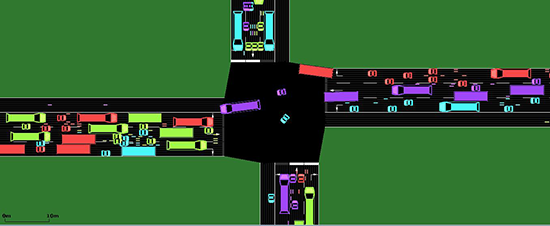
\includegraphics[height=10em]{sumo-1}
    \end{subfigure}
    \hspace{1em}
    \begin{subfigure}[b]{0.45\textwidth}
        \centering
        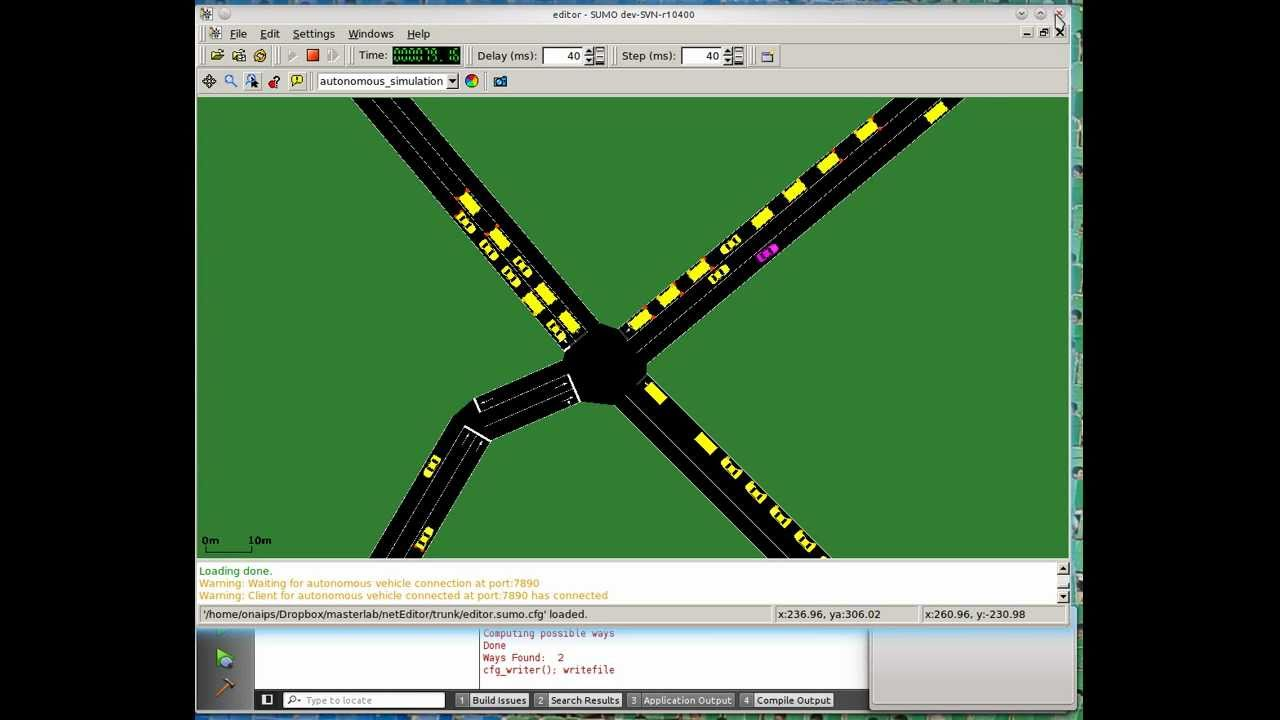
\includegraphics[height=10em,clip,trim=7cm 0 7cm 0]{sumo-2}
    \end{subfigure}
    \caption{Screenshots of the SUMO simulation engine}\label{fig:sumo}
\end{figure}

On the other end of the spectrum, we have SUMO, short for Simulation of Urban
MObility~\cite{sumo}. SUMO is designed for microscopic simulations, down to
individual vehicles and traffic lights. Unlike MATSim, SUMO is a more focused
and unified project (although the default distribution comes with nine pieces of
software), primarily enabling city planners to see the impact of changes to the
road network. Bus timetables and schedules could be changed, traffic lights
added or modified with various models of vehicle behaviour.

SUMO seems to lack many of the issues with MATSim - it is mostly unified,
designed for a specific use case and makes it easy to visualise vehicle
behaviour, as shown in Figure \ref{fig:sumo}. However, SUMO's use cases require
microscopic simulation, meaning it is very accurate for simulating the behaviour
of each vehicle, traffic light, pedestrian and truck. Unsurprisingly, this comes
at a substantial performance cost. SUMO's accuracy and focus makes it a good
tool for its use case, but it does not lend itself to the city scale simulation
and in-depth data analysis that is needed to answer questions about the future
of transportation.

\section{Objectives}

Unlike existing simulation engines, this project aims to create a system
designed exclusively for city-scale real-time macroscopic car simulation, for
aiding development of new multi-vehicle routing algorithms. By focusing on this
use case, we believe a tool can be created that surpasses existing simulation
engines in both performance and ease of use.

\begin{quote}
\noindent
This project aims to have two key deliverables. The first is a flexible, fast
and easy to use simulation and visualisation engine. The second is a
multi-vehicle routing algorithm designed and developed using the simulation
engine. The concrete objectives are:

\begin{enumerate}
    \item Research existing algorithms and simulation tools to identify the
            strengths and weaknesses of current approaches.
    \item Design a simulation architecture that allows for fast experimentation,
        easy integration with real world information and full implementation
        flexibility.
    \item Build and optimise the simulation engine on top of existing open
        source tools.
    \item Design and implement a novel multi-vehicle routing algorithm.
    \item Use the tools provided by the simulation engine to analyse, understand
        and optimise the routing algorithm.
\end{enumerate}

\end{quote}

% -----------------------------------------------------------------------------

\chapter{Technical Background}
\label{chap:technical}

This chapter contains both the algorithmic and practical details that are
required to understand how the project will be delivered. The algorithmic
section covers existing single and multi-vehicle routing algorithms as well as
the processes used for realistic vehicle simulation. The implementation section
introduces the open source software that provides routing algorithms and road
network information to the simulation engine.

\section{Algorithmic Background}

\subsection{Dijkstra's Algorithm}

Dijkstra's Algorithm~\cite{dijkstra}, originally designed in 1956, forms the
foundation of most modern routing algorithms.

\begin{figure}[h]
    \centering
    \includegraphics[page=7,clip,trim=0 10cm 12cm 0,width=0.8\textwidth]{architecture}
    \caption{Graph showing roads with distance and speed limit at the edges}\label{fig:graph-weights}
\end{figure}

The algorithm operates on a graph consisting of nodes connected to each other by
edges. Each edge has a weight, representing the cost of travelling along that
edge. Given a source node $S$ and a destination node $D$, the algorithm returns a list of edges
representing the shortest path between $S$ and $D$.

At its core, the algorithm picks the edge with the next shortest distance from
the source node and updates the minimum distance value for that node. It repeats
this process until it finds the source node, then works backwards to construct
the shortest path between the two nodes.

There are a few key ways of implementing the algorithm, making use of different
types of heap. They each have different performance characteristics, but the
most common approach uses a binary heap and offers $O(E\log V)$ performance,
where $E$ is the number of edges and $V$ is the number of vertices in the graph.

When routing in the real world, the weights of the graph are not usually fixed.
As shown in Figure \ref{fig:graph-weights}, the road's speed limit and distance
are stored on the edges of the graph. This data is used in combination with
information about the vehicle to calculate the travel time, which can then be
used as the weight of an edge. For example, unlike cars motorcycles may not be
able to reach 80mph, so we would use the maximum speed of the vehicle rather
than the road to calculate the travel time for that edge. This concept allows a
single graph to provide routes to multiple types of traveller.

\subsubsection{Bidirectional Dijkstra's Algorithm}

By default, the algorithm searches outwards from only the source. We can improve
the performance of Dijkstra's algorithm by searching backwards from the
destination and forward from the source simultaneously. This has a dramatic
effect on the number of edges that are searched, as can be seen in Figure
\ref{fig:bidijkstra}.

\subsubsection{A* Algorithm}

By itself, Dijkstra's algorithm will search all edges based on their cost from
the start node. However, when routing on a real world map this leads to a lot of
wasted work searching away from the destination - this can be seen in Figure
\ref{fig:bidijkstra}.

Dijkstra's algorithm picks the next edge to check based only on the distance
from the source node, using this as the key in a priority queue. The A*
algorithm modifies this by including a heuristic function representing an
estimate of the distance to the destination node. This allows it to prioritise
nodes that are more likely to route towards the destination. Figure
\ref{fig:astar} shows the paths searched by the A* algorithm - note that it does
not look as far behind the source node as Dijkstra's algorithm, to its left.

A bidirectional version of the A* algorithm can also be used for further
improvements to performance. However, although a bidirectional Dijkstra's
algorithm is significantly more efficient than a single direction one, the same
is not true for the A* algorithm as the heuristics cannot be as
tight~\cite{astar-bi}.

\begin{figure}[h]
\centering
\begin{subfigure}[b]{0.4\textwidth}
    \centering
    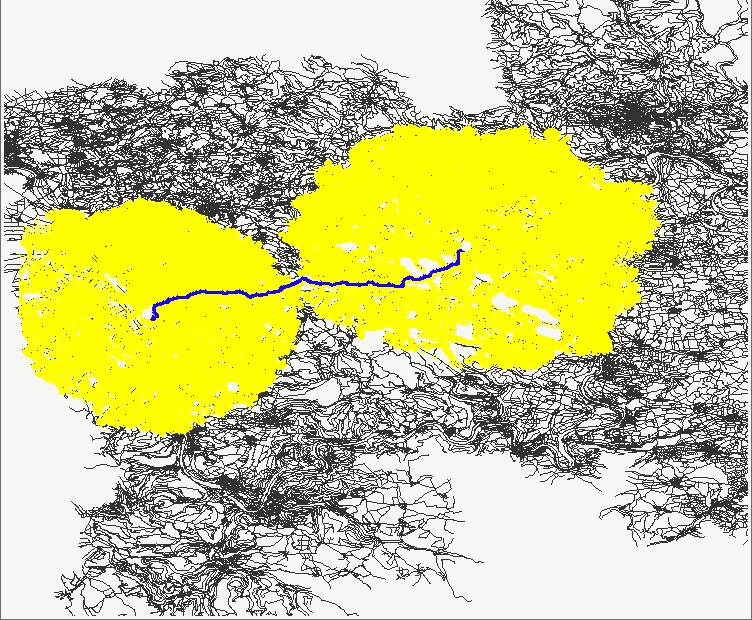
\includegraphics[height=15em]{bidijkstra-city}
    \caption{Bidirectional Dijkstra's Algorithm}\label{fig:bidijkstra}
\end{subfigure}
\hspace{2em}
\begin{subfigure}[b]{0.4\textwidth}
    \centering
    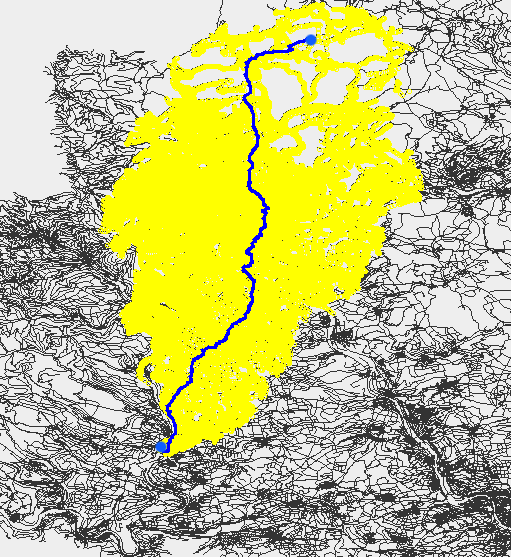
\includegraphics[height=15em]{astar-city}
    \caption{A* Algorithm}\label{fig:astar}
\end{subfigure}
\caption{Paths searched by each algorithm}
\end{figure}

\subsubsection{Contraction Hierarchies}

If the weights on each edge are known in advance, we can pre-process the graph to
compute the shortest path between certain nodes and improve the
performance of routing requests by orders of magnitude. Contraction
Hierarchies~\cite{ch} is one technique for graph preprocessing.  It works by
building shortcuts on top of each other in a hierarchy, and using a modified
bidirectional Dijkstra's algorithm that only uses shortcuts higher than the
current one to route between two points.

Although they double memory usage, in practice Contraction Hierarchies have a
huge impact on query times. For routing from Moscow to Madrid, any Dijkstra
based algorithm takes at least 10 seconds, compared to less than 0.05s for a
processed graph~\cite{ch-perf}.

\subsection{Multi-Vehicle Routing Algorithms}

Providing viable routes for a single vehicle is a problem with accepted
solutions and various implementations used in many successful commercial
products. However, the problem of routing multiple vehicles simultaneously has
many solutions~\cite{beejama,rt:compstudy,rt:decentralized,
rt:guidance,rt:congestion,rt:car,rt:unexpected}, but no accepted `best practice'
technique.

This is primarily due to their research focussed nature - it is not currently
possible to route all vehicles collaboratively, so many types of algorithm exist
to deal with different expectations of the future of transport communication.

As such, multi-vehicle routing algorithms usually fall into one of two
categories. Some algorithms are designed to have a large scale overview of where
each vehicle is on the road using some secondary infrastructure, and will
dispatch routing information to the vehicles centrally. On the other end,
algorithms may assume no central information and instead rely upon vehicle to
vehicle connections for passing information. Algorithms relying on the
installation of additional infrastructure are referred to as \textbf{V2I},
standing for Vehicle to Infrastructure, whilst \textbf{V2V} refers to Vehicle to
Vehicle algorithms. A simulation engine capable of implementing both V2V and V2I
communication models is known as a V2X engine.

\subsubsection{VANET}

A VANET (Vehicular-AdHoc NETwork) is a high-level use of V2V communication.
Although primarily theoretical at the moment, wireless networking protocols and
algorithms have been designed to support the creation and use of a VANET. VANETs
have a number of potential use cases - allowing vehicles to follow one another
with no driver intervention, real-time calculation and distribution of traffic
information and so on. V2V algorithms relying on a VANET have been created and
shown to offer improvements in routing performance.

\subsubsection{BeeJamA}\label{sec:beejama}

\begin{wrapfigure}{r}{0.4\textwidth}
    \vspace{-1em}
    \begin{greybox}
        \centering
        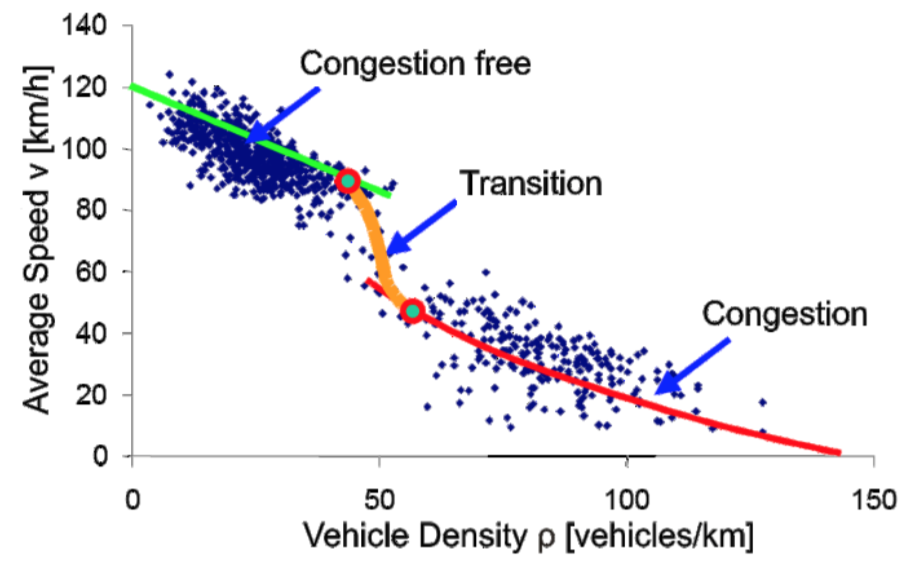
\includegraphics[width=\textwidth]{congestion-graph-1}
        \caption{Empirically derived congestion function from~\cite{traffic-graphs}}\label{fig:congestion-graph}
    \end{greybox}
    \vspace{-3em}
\end{wrapfigure}

The BeeJamA~\cite{beejama} algorithm is a V2I approach for multi-vehicle routing. It is based
off an algorithm originally created for routing in packet switching networks
that has been adapted for use on road networks. Its behaviour is inspired by the
behaviour of bees, which are able to effectively search and scavenge for food in
a large area surrounding their hive.

The map is split into regions called Foraging Regions. Each region stores two
types of table - an Intra-Foraging Region routing table and an Inter-Foraging
Region routing table.  These store the cost of using a particular route to reach
the destination. The tables are kept up to date by sending virtual vehicles
between regions, which record how long their journey took and update the tables
of the region they have entered.

Whilst routing, each vehicle consults the routing table and probablistically
picks its next step. This is a key part of the algorithm that helps keep routes
uncongested - if every vehicle took the optimal path, it would no longer be
optimal as it would have high levels of congestion. Results from a custom-built
simulation engine have shown that the algorithm can perform better than using
Dijkstra's algorithm with delayed traffic information.

\begin{wrapfigure}{r}{0.4\textwidth}
    \vspace{-1em}
    \begin{greybox}
        \centering
        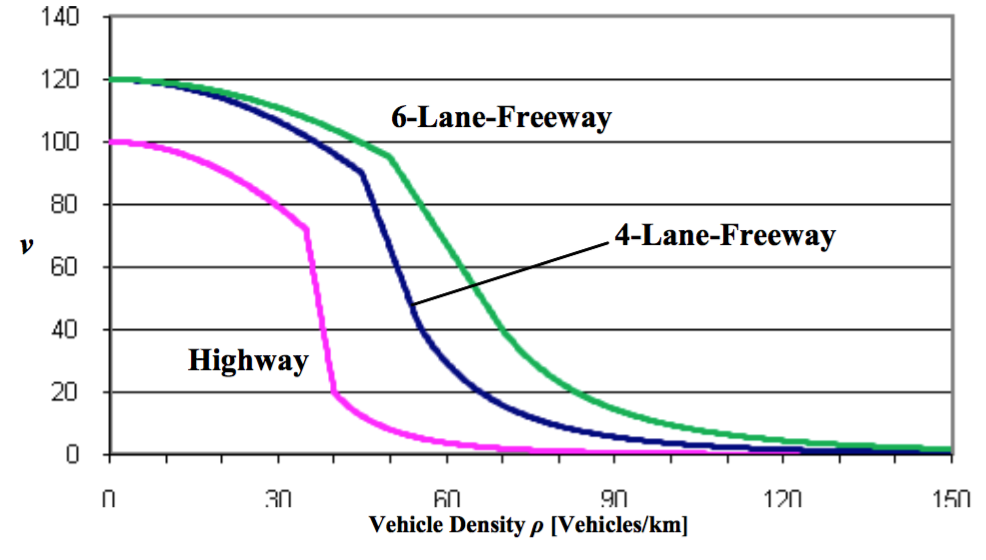
\includegraphics[width=\textwidth]{congestion-graph-2}
        \caption{Mathematical congestion functions for different types of road from~\cite{beejama}}\label{fig:congestion-graph-2}
    \end{greybox}
    \vspace{-3em}
\end{wrapfigure}

When routing with Dijkstra's algorithm, the travel time for each edge is usually
estimated based only on the road's speed limit and distance (as well as the
maximum speed of the vehicle). The BeeJamA improves upon this drastically by
taking into account the number of vehicles on a given road. Instead of using the
maximum velocity for a road, BeeJamA uses a congestion function that takes into
account the density of vehicles on a given road as well as the road type. The
congestion functions they and other researchers have derived can be seen in
Figures \ref{fig:congestion-graph} and \ref{fig:congestion-graph-2}.

Empirical analysis of real world data has been performed with the goal of
creating a function from density of vehicles to velocity~\cite{traffic-graphs,
traffic-thing-2}.

\subsection{Nagel-Schreckenberg Model} \label{sec:nagel}

The Nagel-Schreckenberg Model~\cite{nagel} is a cellular automaton model for the
flow of traffic on roads.

The model splits roads into discrete cells, with each car taking up a single
cell at a time. The vehicles then follow 4 rules to simulate the flow of
traffic. Each car has a fixed velocity $v$, which represents the number of cells
the vehicle intends to move forward. The first three steps determine the
velocity, with the final step updating the position of each vehicle.  The model
does not allow for overtaking, exhibiting realistic behaviour for traffic jams
and flow.

\begin{enumerate}
    \item \textbf{Acceleration} - if the vehicle is not at the max speed and
        there is enough space ahead, increase the velocity by 1.
    \item \textbf{Slowing down} - if there is a vehicle nearer than the current
        velocity, reduce velocity to one cell less than the distance to the
        vehicle in front.
    \item \textbf{Randomisation} - reduce the velocity by 1 with probability
        $p$.
    \item \textbf{Movement} - move each vehicle forward by its velocity $v$.
\end{enumerate}

Each cell is meant to approximately represent the size of a single vehicle,
whilst each step (running through all four rules) represents a discrete amount
of time - usually a single second.

We'll now run through a brief example of the effects of each step. Our road will
have nine cells and two vehicles. Our max speed ($v_{max}$) will be 5.  For this
example, we will ignore the randomisation step.

\begin{figure}[!h]
\centering
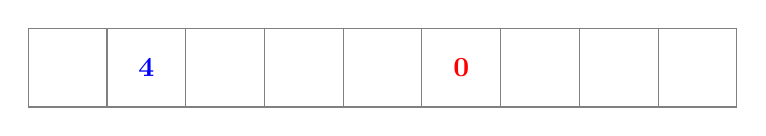
\begin{tikzpicture}
    \draw[step=1cm,color=gray] (0,0) grid (9,1);
    \node at (1.5,0.5) {\color{blue} \textbf{4}};
    \node at (5.5,0.5) {\color{red}  \textbf{0}};
\end{tikzpicture}
\end{figure}

We first perform the acceleration step for each vehicle. The blue vehicle
is currently at speed 4 - as the red vehicle is only 3 cells away, it does
not increse its velocity. The red vehicle increments its speed from 0 to 1.

During the slow step, the blue vehicle must reduce its speed from 4 to 3
so it does not hit the red vehicle.

\begin{figure}[!h]
\centering
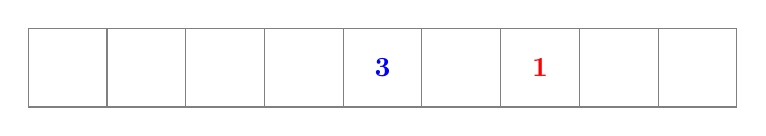
\begin{tikzpicture}
    \draw[step=1cm,color=gray] (0,0) grid (9,1);
    \node at (4.5,0.5) {\color{blue} \textbf{3}};
    \node at (6.5,0.5) {\color{red}  \textbf{1}};
\end{tikzpicture}
\end{figure}

The vehicles now move to their new destinations. This demonstration briefly
shows the interaction between two vehicles, but does not demonstrate the
creation and flow of traffic jams. In Figure \ref{nagel-demo}, we can see how
traffic jams form and move in the Nagel-Schreckenberg model. This graph shows
what happens when there is a density of 0.1 cars per cell.

\begin{figure}[h]
    \centering
    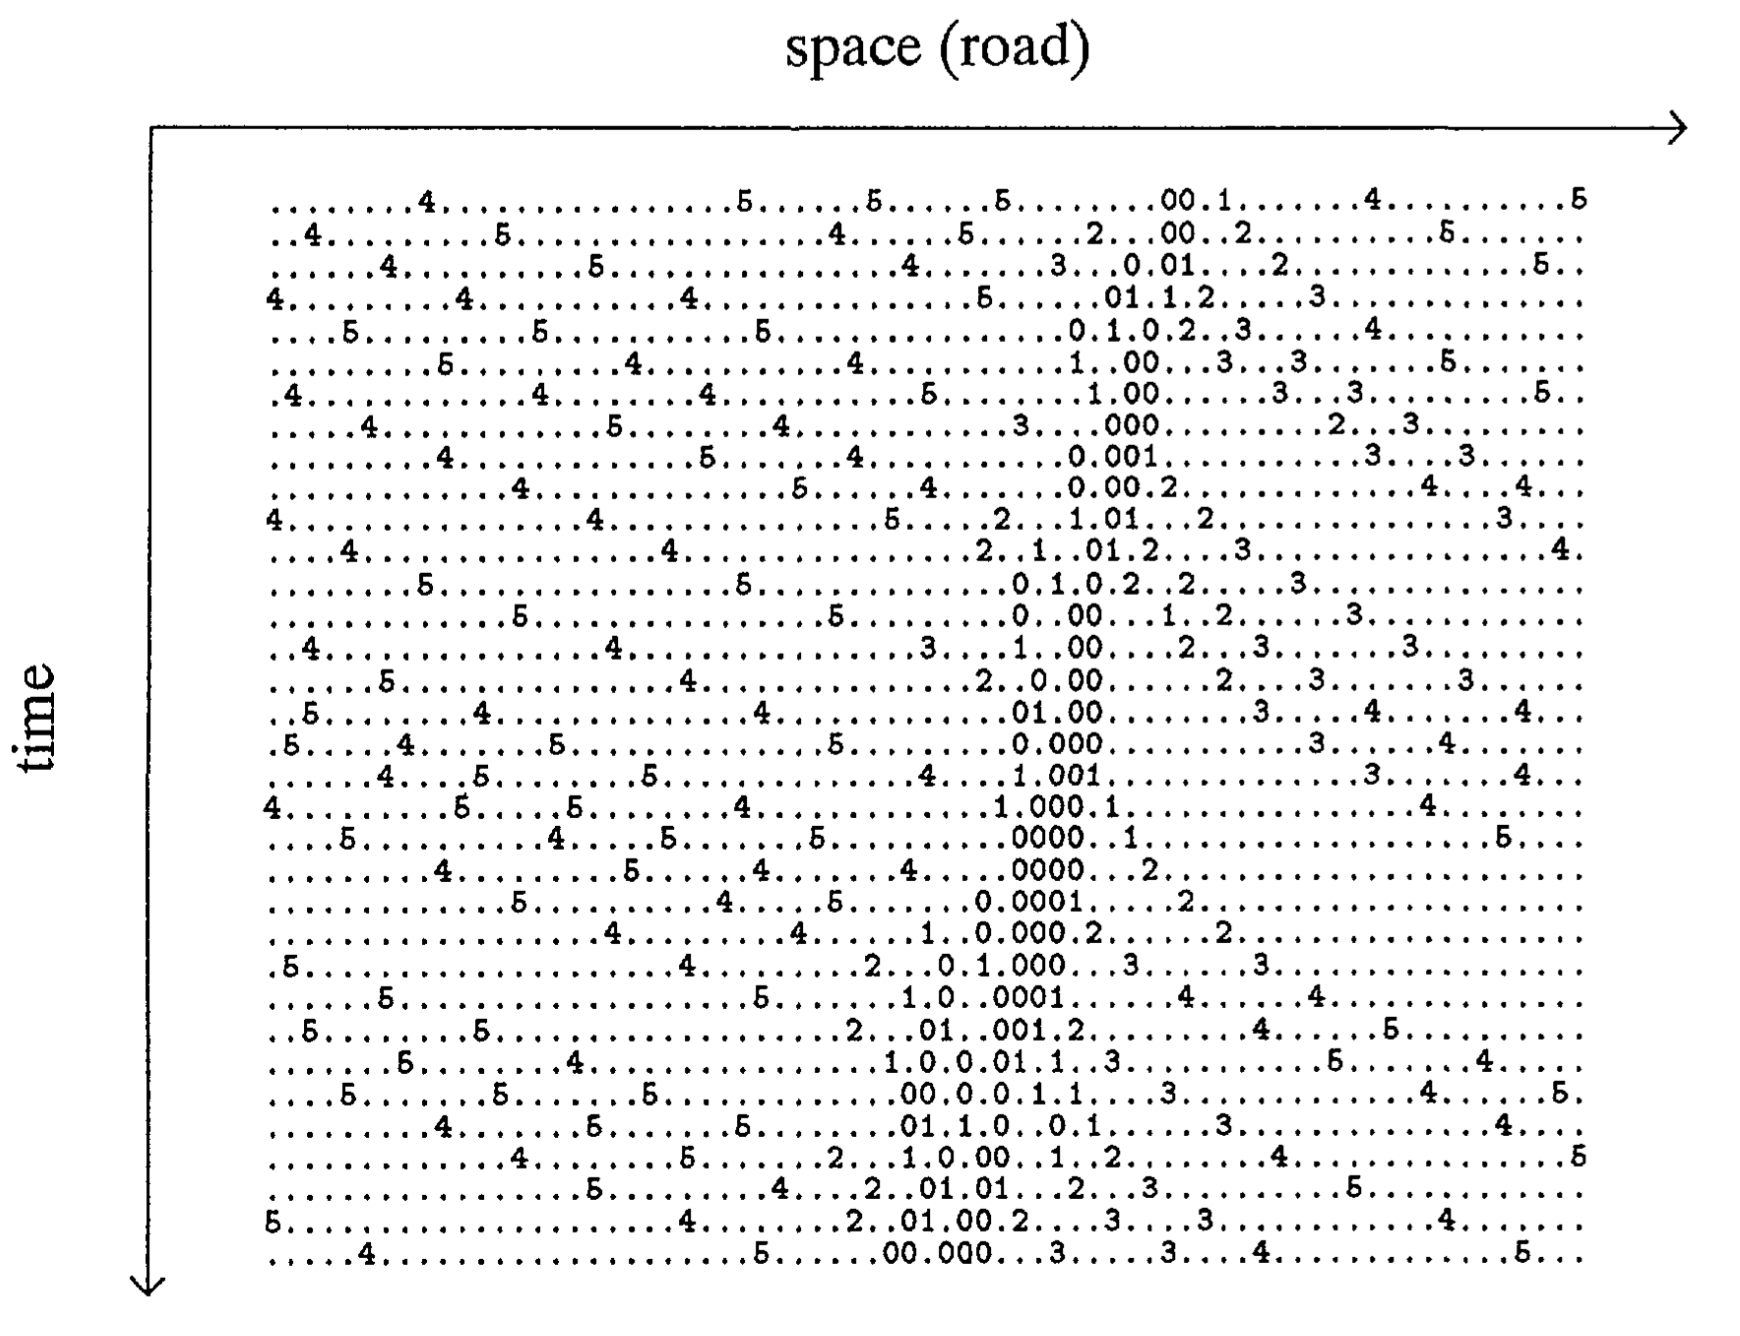
\includegraphics[scale=0.4]{nagel}
    \caption{Formation of traffic jams in the Nagel-Schreckenberg Model
    from~\cite{nagel}}\label{nagel-demo}
\end{figure}

\section{Implementation Background}

\subsection{OpenStreetMaps}

In OpenStreetMaps, there are three main elements - nodes, ways, and relations.
Each of these can have certain tags that describe the real-world object they
represent. For example, a way could have tags describing it as a highway with 3
lanes, whilst a node could have tags identifying it as a park bench or phone
booth.

A standalone node is usually a single entity with a latitude and longitude as
well as an ID. By themselves, they can be used to represent small features such
as traffic lights, lampposts, or pylons. However, a way is also defined by an
ordered list of nodes.

Ways are the most flexible element in OpenStreetMaps. If a way starts and ends
at two different nodes, it is called an `open' way. This is commonly used for
sections of roads and paths. A way that starts and ends at the same node is
called a `closed' way. Often this is used to represent an area - such as a park
or the shape of a building - but can also be used for roundabouts and circular
barriers. There are tags for identifying if a closed way is an area or not
(primarily the \texttt{area=yes} tag, but many things are defined as areas even
without this tag).

Finally we have relations. These are the most complex type of element, holding
an ordered list of ways, nodes and other relations and have tags for describing
the relationship between them - for example, a bus route could be described as a
list of ways and nodes. For the purposes of routing, it is only important to
know that relations are used for turn restrictions - the rules that define which
directions a vehicle may move from one road onto another. This is important for
routing much more than mapping, as users would be frustrated to find that a
route they had expected to travel on is illegal or unsafe in practice.

\subsection{GraphHopper Routing Engine}

GraphHopper has been built to be fast, flexible and powerful. It covers the full
flow of creating a custom routing service - from parsing and importing
OpenStreetMaps data, processing the network for performance improvements,
routing using multiple Dijkstra and A* algorithms and running a web server for
making requests. Additionally, it has built in support for car, bicycle,
pedestrian and other types of travel as well as the ability to create custom
vehicle types.

\begin{figure}[p]
    \centering
    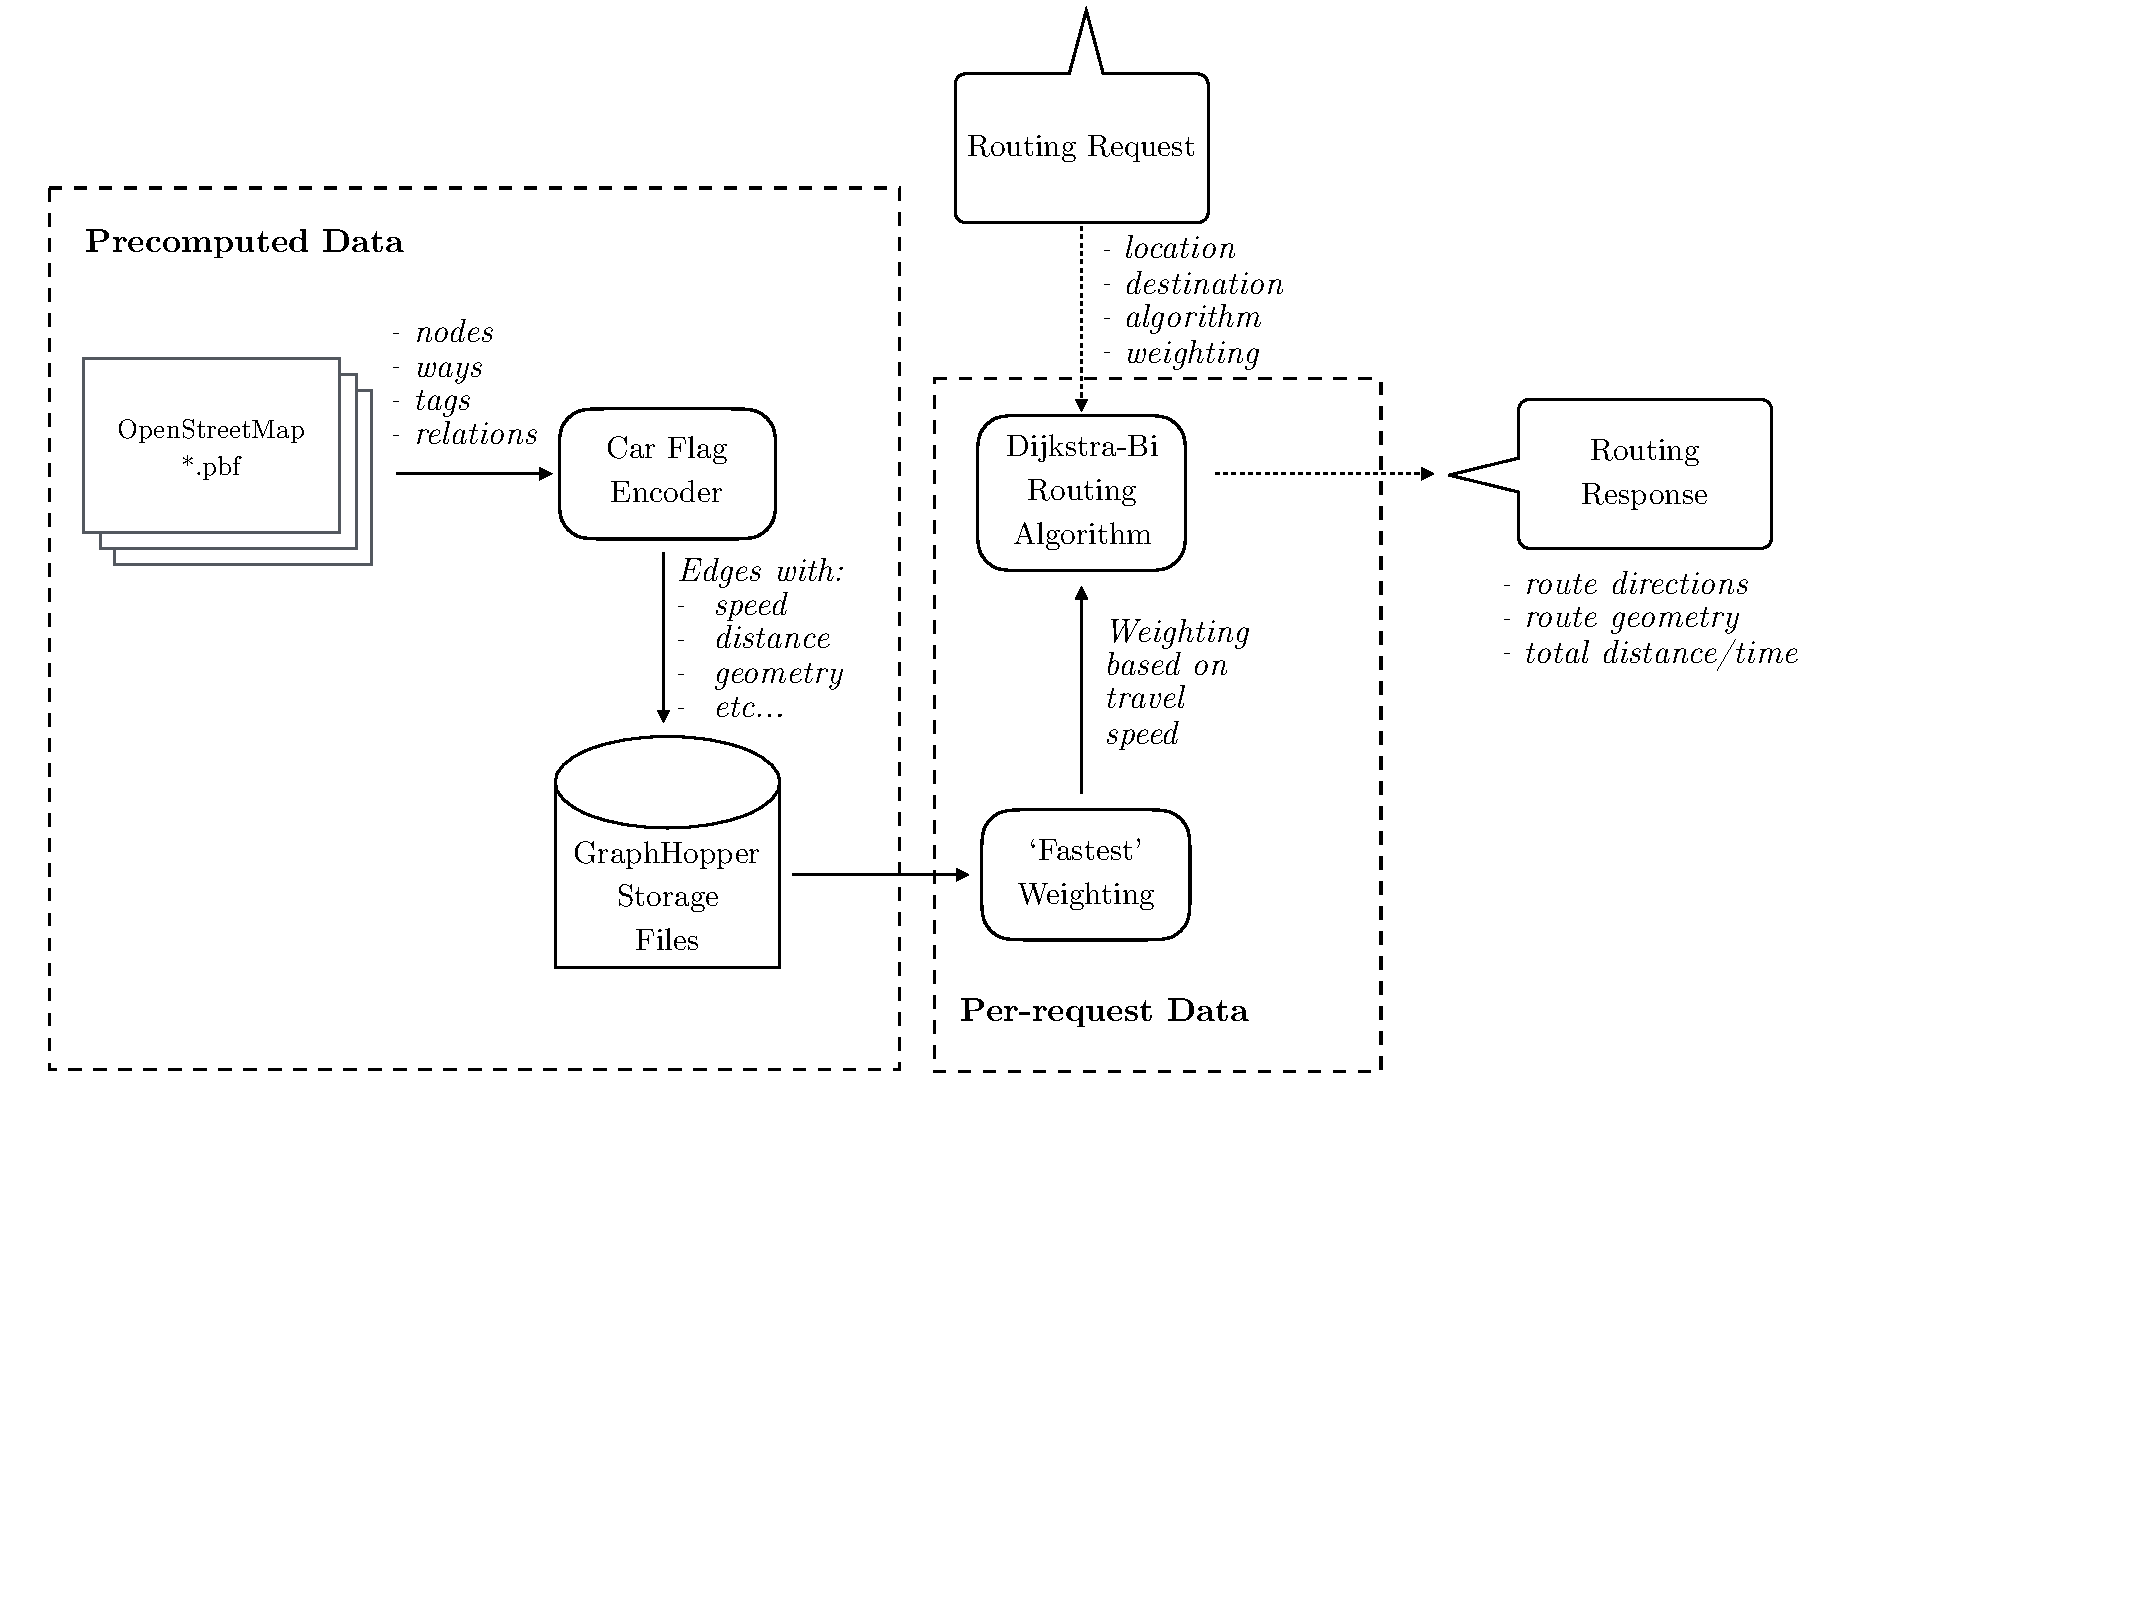
\includegraphics[scale=0.5,page=1,clip,trim=0 8cm 4cm 0]{architecture}
    \caption{An overview of the GraphHopper Architecture}\label{fig:gh-arch}
\end{figure}

Figure \ref{fig:gh-arch} shows the salient parts of the architecture for this
project.  Note that we are not using the web or android modules, so no details
regarding their functionality has been included. For the most part, the use of
routing will be relatively high level - simply requesting a list of edges
between two points. However, the underlying engine also has a number of features
that make it easy to customise, which will be used for more complex situations.

It is important to note that the conversion from OSM data to GraphHopper data is
done only once (as it is a time consuming process) and stores its results on
disk.

\subsubsection{OpenStreetMap Encoding}

\begin{figure}[p]
    \centering
    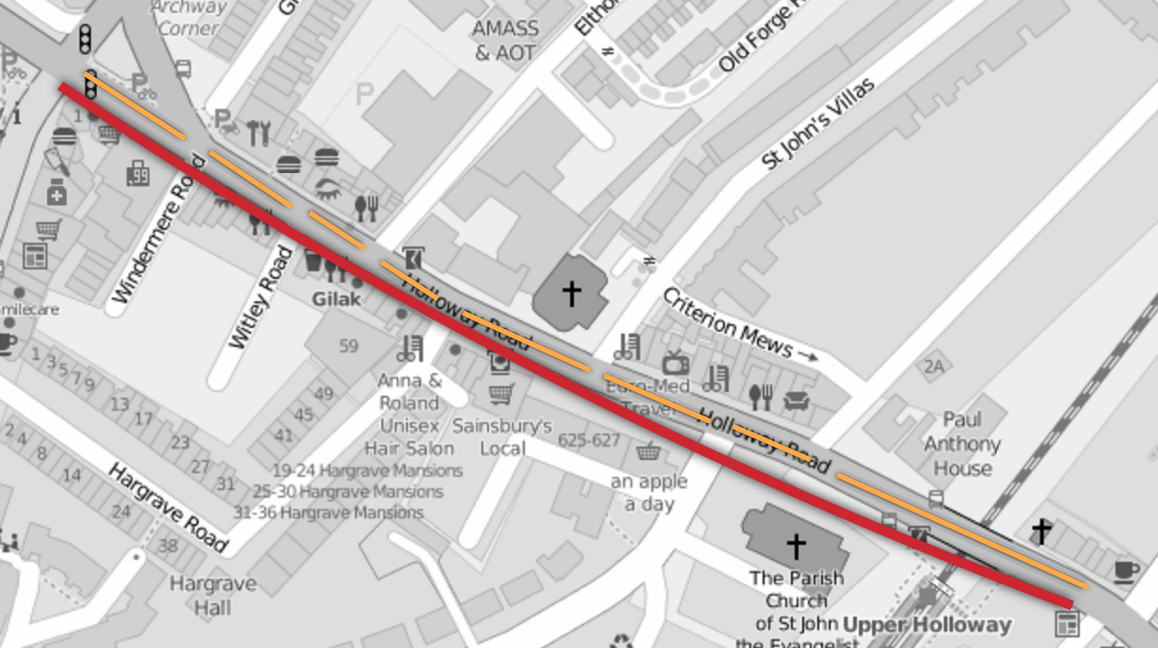
\includegraphics[scale=0.6]{osm-gh}
    \caption{OpenStreetMap way representation compared to edges in GraphHopper}\label{fig:osm-gh}
\end{figure}

The first thing to understand is how GraphHopper converts the OpenStreetMap data
into a graph that can be used for routing.  For the purposes of routing, we are
primarily concerned with ways that represent roads. However, a way does not
represent the entirety of a given road - but is also not granular enough to
allow routing. Figure \ref{fig:osm-gh} shows the difference between ways, roads
and edges. We can see that the physical Holloway Road extends beyond the OSM way
(red). However, if we used the way for routing we could not route from Hargrave
Road to St John's Villas via Holloway Road. To perform routing, GraphHopper
splits every way into an edge whenever there is a junction. GraphHopper's edges
can be seen in orange. These can be used to perform the routing calculation
mentioned above - there is now an edge along a subsection of Holloway Road that
connects Hargrave Road to St John's Villas.

\subsubsection{Flag Encoders}

Internally, GraphHopper compresses the information about each edge into a single
integer - so each edge takes up no more than 32 or 64 bits.

The \texttt{FlagEncoder} interface (and the \texttt{AbstractFlagEncoder} class)
define what operations have to be done to convert a section of a way into an
edge. Edges store a few key pieces of information - by default, GraphHopper
stores the length, speed and ID of an edge, with additional information
optionally stored by the flag encoder itself.

For example, the \texttt{CarFlagEncoder} uses the type of road to calculate the
correct maximum speed of the vehicle and then sets the speed for the edge, using
5 bits. The \texttt{MotorcycleFlagEncoder} can do the same thing, but with
different speed values for each type of road. The concept can be extended to
storing even more information at each edge - for example, 3D graph data can be
stored for bike and walking routes, whilst a FlagEncoder for trucks could store
height, weight, width and length restrictions to ensure safe travel.

\subsubsection{Weightings}\label{sec:gh-weighting}

Flag Encoders are used to define what information can be used whilst routing -
but this data is fixed once the OSM file has been processed. A weighting defines
how the data stored at the edges is used. For example, one can search for the
shortest route, the fastest route, or a custom weighting that incorporates other
information stored in the edge.

\subsubsection{Routing Requests}

As it is primarily designed to work with its web module, GraphHopper uses a
request-response pattern for requesting and receiving routes.

\begin{lstlisting}[label=lst:gh-route,caption={GraphHopper request and response}]

GHRequest ghRequest = new GHRequest(startLat, startLon, endLat, endLon);
ghRequest.setWeighting("fastest");
ghRequest.setAlgorithm("dijkstrabi");
GHResponse ghResponse = graphHopper.route(ghRequest);

\end{lstlisting}

The \texttt{GHRequest} class stores all the information required to make a
routing request, including the weighting and algorithm to use. An example of its
use can be seen in Listing \ref{lst:gh-route}.

The response is returned in a \texttt{GHResponse} class, which holds information
about the route in a number of different ways. The user is also responsible for
checking the \texttt{hasErrors} method before requesting the route itself.  Once
this has been done, the route itself can be read.

As GraphHopper supports the use of an alternative routes algorithm (meaning a
single request can respond with more than one route), the GHResponse class has
both a \texttt{getAll} and \texttt{getBest} method, which return a list of
\texttt{PathWrapper}s and a single PathWrapper respectively. The PathWrapper
holds the route itself as well as some metadata. The route can be accessed as a
list of instructions or as the raw list of points for visual display.
Additionally, the total distance and time of the route are recorded.

However, GraphHopper does not provide a list of edges or of OSM Ways that are
included in the route. Internally, the list of edges is calculated with the
\texttt{calcPaths} function, which returns a list of \texttt{EdgeIteratorState}
objects. These objects are fundamental to the way the graph is stored an
accessed in GraphHopper.

GraphHopper uses the flywheel pattern for efficient access to graph data. The
EdgeIterator and EdgeIteratorState class are the primary way of interacting
directly with the edge data. EdgeIteratorState is an interface containing
getters and setters for the edge ID, its geometry, the flags stored by the
FlagEncoder, and the name of the road the edge is a part of. It also allows
access to the nodes at either end of this edge. The node at the start of the
edge is called the Base Node, whilst the node at the end of the edge is the
Adjacent Node.

% -----------------------------------------------------------------------------

\chapter{Project Execution}
\label{chap:execution}

\section{Overview}

The execution of this project was split into 4 stages, each with its own goal.

\begin{enumerate}
    \item \textbf{Initial Implementation} - create the initial client and
        server with vehicles moving on a map.
    \item \textbf{Realistic Simulation} - implement the Nagel-Schreckenberg
        model to make the vehicle behaviour more realistic.
    \item \textbf{Performance and Architecture Improvement} - make the
        simulation engine fast and flexible enough to deal with the challenges
        of algorithm design.
    \item \textbf{Algorithm Design and Implementation} - create and improve
        a novel approach to the multi-vehicle routing problem using the
        simulation engine.
\end{enumerate}

\section{Initial Implementation}

The initial implementation had a few key goals, with a primary objective of
showing basic vehicles moving on a map. This stage was essentially a way of
setting up the basic architecture of the project, without finalising the
details of how routing algorithms would be implemented.

\subsection{Architecture Design}

\begin{figure}[h]
    \centering
    \includegraphics[scale=0.5,page=2,clip,trim=0 17cm 3cm 0]{architecture}
    \caption{The initial architecture for the simulation engine}\label{fig:init-arch}
\end{figure}

Figure \ref{fig:init-arch} shows a simple architecture diagram for the initial
implementation of the engine. Once the client has made a request, the engine,
sets up and starts routing the vehicles. Each vehicle is responsible for storing
and updating its own position on each timestep. This data is converted into a
string and sent to the client, which then moves each vehicle on the map.

One of the goals of this project was to make it possible to visualise and
simulate the vehicles at the same time. This naturally lends itself to a
client-server architecture, and with the rate of improvement of modern web
browsers it seemed like a wise choice to use a browser for the visualisation
component.

This also means that the server can be run remotely with no additional setup -
more computationally expensive algorithms could be run on high-powered servers
with the results still visible locally for the user.

\subsection{Project Setup and Modularisation}

When setting up the project, it was important to be able to use and modify the
underlying GraphHopper routing engine. The GraphHopper project is setup with
four existing modules - \texttt{core}, \texttt{tools}, \texttt{web}, and
\texttt{android}. Although it would have been ideal to use GraphHopper as an
external library, it was necessary to make minor internal changes to the main
engine. As such, a GitHub fork of the project was created with \texttt{marmoset}
as a fifth module in the project.

GraphHopper uses the Maven dependency and build tool, with its own custom shell
script for building, running and testing different versions of the engine. To
keep Marmoset separated from the core project, a custom shell script for
building and running the Marmoset engine was created. It supports four main
actions - clean, build, rebuild, and run. It also allows multiple commands to be
run in succession for convenience.

Additionally, it was desirable to create a modern codebase in spite of the core
engine being written in Java. Although Scala was briefly considered, much of my
work would rely on extending and using the existing Java APIs in GraphHopper.
Thankfully, Java 8 has introduced a number of key tools that allow
functional-style code to be written. The code below shows the difference for
performing a simple task - converting a list of objects into strings and joining
them by commas.

\noindent
\begin{tabular}{c|c}
\begin{lstlisting}
public String getVehicleData()
{
    StringBuilder sb = new StringBuilder();
    for (VehicleController v : vehicles)
    {
        sb.append(v.getVehicle().toString());
        sb.append(",");
    }
    // remove last comma
    sb.deleteCharAt(sb.length() - 1);
    return sb.toString();
}
\end{lstlisting} &
\begin{lstlisting}[boxpos=b]
public String getVehicleString()
{
    return vehicles.stream()
        .map(Vehicle::toString)
        .collect(Collectors.joining(","));
}
\end{lstlisting} \\ \vspace{1em}
Java 7 Implementation & Java 8 Implementation \\
\end{tabular}

Here we can see how six lines of code can be condensed into a single, more
readable line using the Java 8 Stream API.

\subsection{Server Implementation}

For the raw file server, the NanoHttd~\cite{nanohttpd} library was used, as it
requires minimal setup and is easy to run on a separate thread. For the
client-server communication, initially the NanoHttpd WebSocket implementation
was used, but it did not appear to be fully functional. As such, the
Java-Websocket library~\cite{javawebsocket} was used instead, extending the
built in WebSocketServer class to create the \texttt{MarmosetSocketServer} class.

In the architecture diagram (Figure \ref{fig:init-arch}), we see four main
classes on the back-end.

The \texttt{MarmosetSocketServer} class handles the connection between server
and client.  It keeps track of each of the connected clients and offers a simple
command to distribute vehicle position data to each of them.

The \texttt{Marmoset} class is a static class, and is the main entry point for
the program. It initialises the file server and WebSocket server, and creates a
new thread for running the \texttt{MarmosetHopper} timesteps. It also handles
passing data from \texttt{MarmosetHopper} to the socket server.

In most types of simulation, time must be split into discrete steps that
represent a fixed time interval in the real world. Looking at Figure
\ref{fig:init-arch}, we can see that it is the Marmoset class that triggers each
timestep. At this stage of the project, it had not been established how
effectively the front or back end would perform at receiving and rendering the
vehicles. As a way of simplifying the data flow and processing, the Marmoset
class simply waits one second between each call of the timestep function.  As
both front end and back end take significantly less than a second to perform
their tasks, this was an appropriate simplification for this stage of
development.

The \texttt{MarmosetHopper} class holds the list of vehicles and creates an
instance of the GraphHopper routing engine. It initialises all the vehicles,
instructs them to update on each timestep, and gathers their position
information together to be sent to the clients. When initialising the vehicles,
the starting location and destination are chosen as random latitude and
longitude co-ordinates within London.

Finally, the \texttt{Vehicle} class represents a single physical vehicle on the
map. Each vehicle holds its location and the route it plans to take. The routing
information is obtained by requesting a route from GraphHopper. The route is
returned in a number of ways, including as a list of points that can be used to
draw the route. This does not include the speed of each road travelled, so
cannot be used for realistic simulation. However, for this initial
implementation the location is updated on each timestep by simply moving to the
next point in the list. This is not realistic, but it does allow us to verify
the functionality of all parts of the system without touching the details of
routing. The vehicles return their location as a string containing their ID,
latitude and longitude.

\subsection{Client Implementation}

When loading the web page, a map is created and centred on central London.  The
client then connects to the WebSocket back end and listens for data. When it
receives the vehicle data, it creates or updates the position of each vehicle
marker.

The Leaflet.js~\cite{leaflet} library is used for both map and marker creation.
A simple \texttt{Car} class has been created to keep track of the location of
each marker. It stores a reference to the Leaflet.js Marker object and provides
a method to move the marker to a new location. The
Leaflet.AnimatedMarker~\cite{animarker} library handles smoothly moving the
points to their next location, making the cars look like they are driving around
the map in real-time.

Meanwhile, a single \texttt{CarSet} object connects to the WebSocket server and
stores the \texttt{Car} objects. When data is received, it creates new
\texttt{Car} objects or updates the position of existing vehicles using their
\texttt{moveTo} method.

\subsection{Results and Improvements}

\begin{figure}[h]
\centering
\begin{subfigure}[b]{0.4\textwidth}
    \centering
    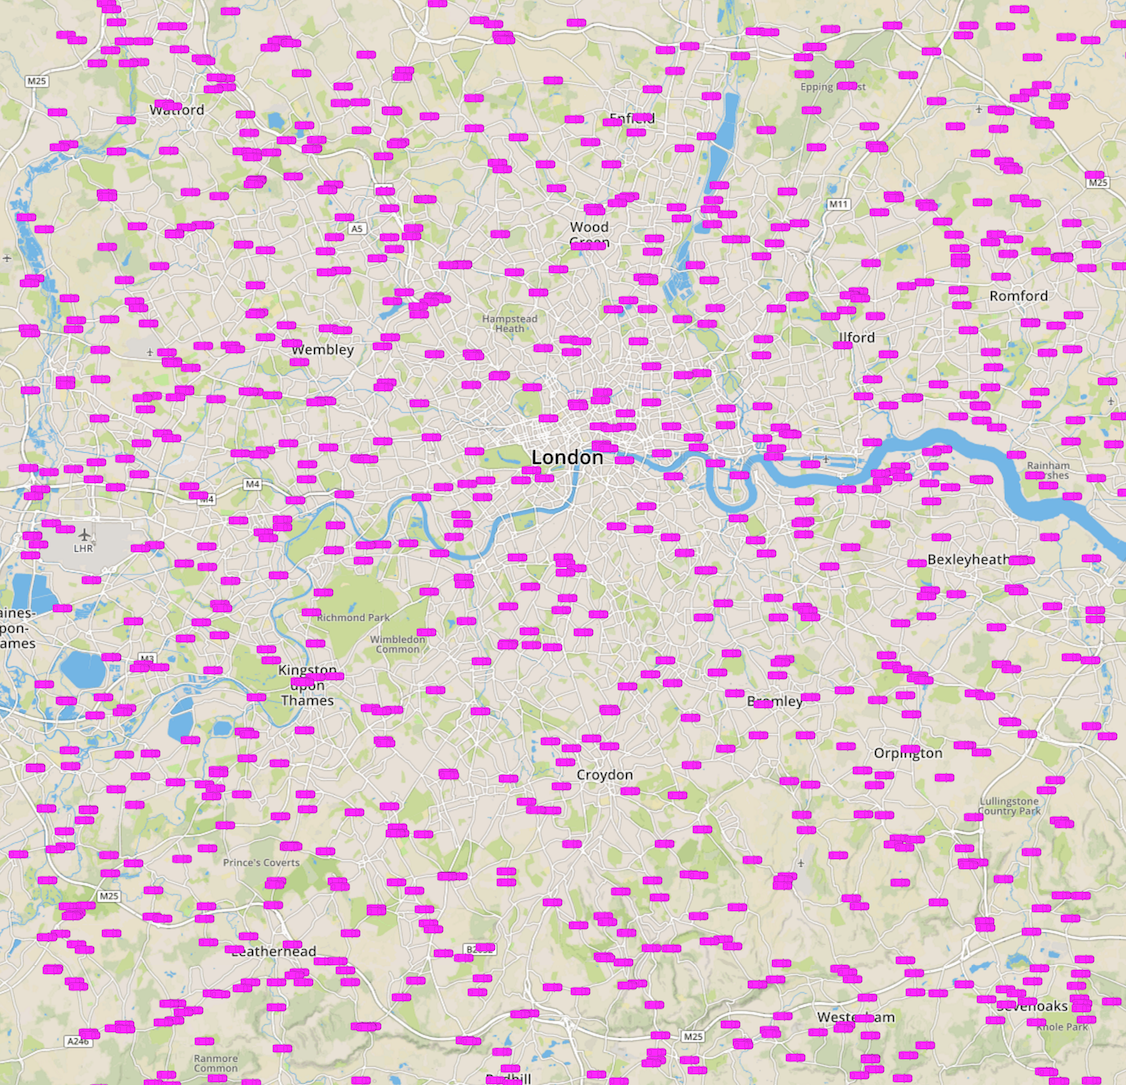
\includegraphics[height=15em]{init-start}
    \caption{10th Iteration}\label{fig:init-start}
\end{subfigure}
\hspace{2em}
\begin{subfigure}[b]{0.4\textwidth}
    \centering
    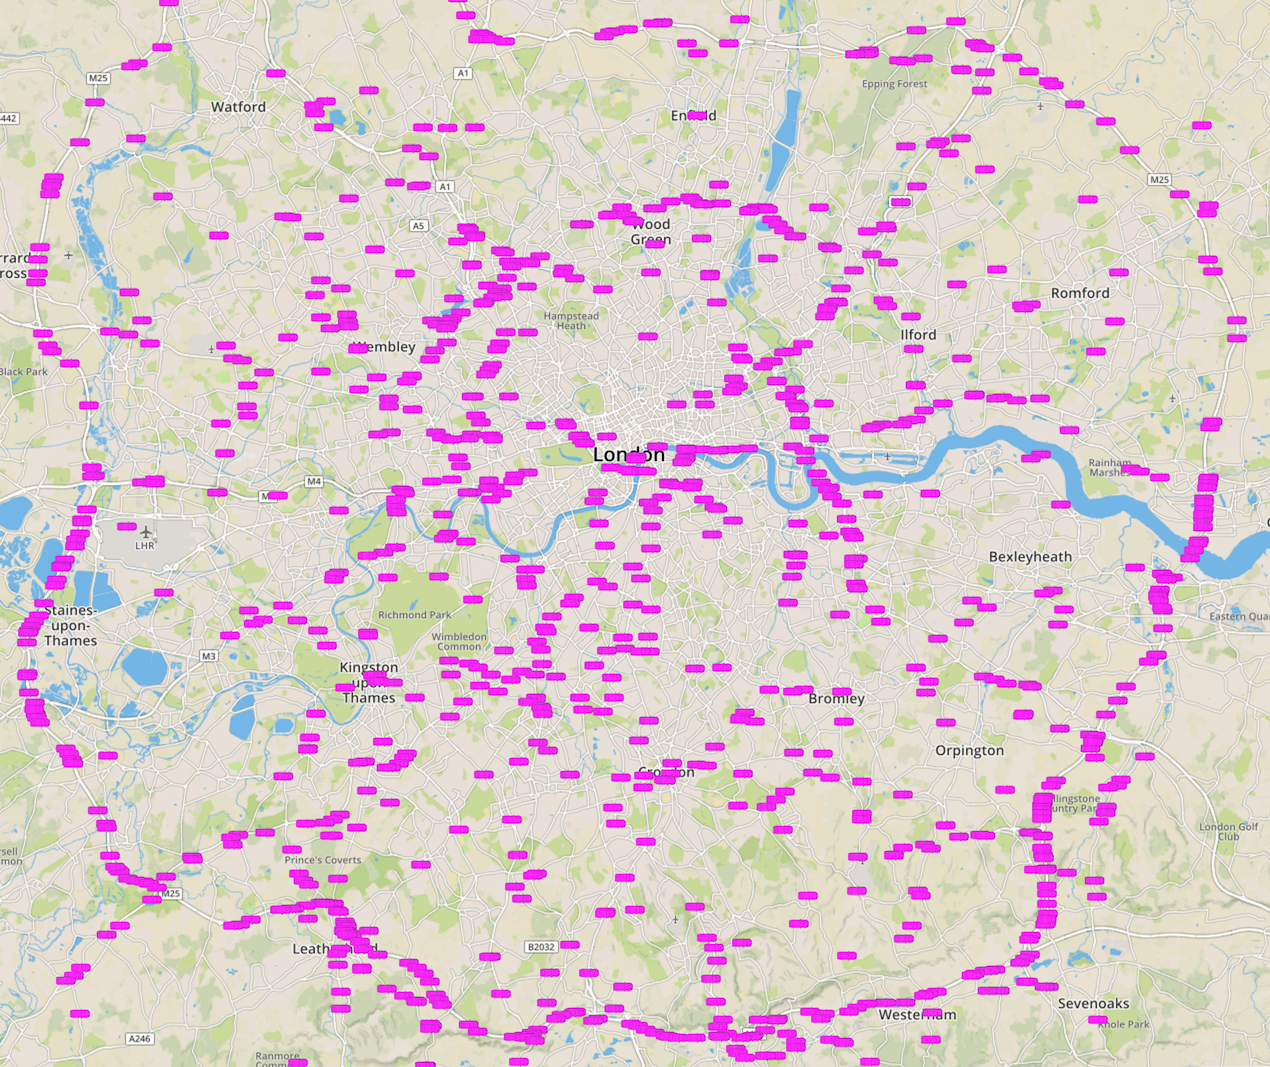
\includegraphics[height=15em]{init-200}
    \caption{200th Iteration}\label{fig:init-200}
\end{subfigure}
\caption{Vehicle positions at different iterations}
\end{figure}

At the end of this section of the project, the engine was capable of performing
its core task of simulating and visualising vehicles. In spite of many of the
simplifications in the system, it provides quite realistic results -
\ref{fig:init-200} shows that even after a small number of iterations certain
roads become more congested than others. This matches the reality of driving on
London roads - the M25 and North Circular suffer frequent delays due to high
levels of congestion.

However, there are many core features missing from the engine at this point:

\begin{itemize}
    \item The engine simulates a fixed number of vehicles (1000); no more can
        be added or removed.
    \item Vehicles do not move realistically; as they simply jump to the next
        point on their route, a short curved path would take longer to
        travel along than a long but straight motorway.
    \item Vehicles are independent, travelling on their own with no sense
        of traffic or congestion.
    \item The timestep is fixed to one second, even though the actual processing
        takes substantially less time for both front and back end.
    \item Metrics are not tracked; other than watching the simulation, there is
        no further understanding that can be gained from simulating.
    \item The simulation cannot be paused without terminating it and starting
        again.
\end{itemize}

The focus for the next stage of develeopment was on improving the realism of the
vehicle simulation.

\section{Realistic Simulation}

In section \ref{sec:nagel} we introduced the Nagel-Schreckenberg Model for
traffic flow simulation. This section discusses the implementation of this model
on top of the existing simulation engine described above.

The original model is designed for a single road, either in a loop or an
extended straight stretch. Implementing this on a road network introduces some
additional challenges, particularly when handling the integration between
GraphHopper and OpenStreetMaps.

The two main concerns are how the cells should be stored and how the cells
should be used in conjunction with the routes created by GraphHopper.

\subsection{Cell Storage}

A number of techniques for storing the cells were considered. Firstly, we must
consider how we create edges. We have the option of using either GraphHopper
edges - which are small, but do not have junctions - or OSM ways, which can be
larger but would allow for more usable metrics and would make the system less
dependent on GraphHopper.

Ultimately, GraphHopper's edges were chosen as the base unit for cells. This was
primarily due to the fact that GraphHopper does not have an internal mapping
from its edges to OSM Ways, and does not return which Ways are used as part of a
routing response. Additionally, GraphHopper provides an
\texttt{AllEdgesIterator} that returns both the maximum edge ID as well as the
data for every edge in the graph.

The next decision was how and where to store the cells. In the original paper, we
saw that each vehicle was represented by its velocity stored as an integer in
the cell array. As we are storing a much larger amount of information about each
vehicle in the Vehicle class, this is not a viable option. If vehicles store
their own velocity and keep track of the current edge and cell they are on, the
cells only need to know if any vehicle is present in a cell. As such, each cell
is simply a boolean value in an array. The cell is set to \texttt{true} if a
vehicle is in the cell and \texttt{false} if the cell is empty.

In terms of physical storage, the are a number of options. At its core, we need
a mapping from edge IDs to cell arrays. In Java, this would usually be
represented as a Map of Lists (\texttt{Map<Integer, List<Boolean>>}). However,
the edge IDs in GraphHopper have been designed to be sequential starting from 0,
with the highest ID accessible from the \texttt{AllEdgesIterator}. This means
that we can instead use a list of lists (\texttt{List<List<Boolean>>}). This has
the advantage of allowing the lists to grow in size dynamically, but may have
performance issues. In Java, Lists must store other Object types rather than
primitive types. As objects in Java are all pointers, each Boolean will require
a pointer to a separate memory location that holds the \texttt{true} or
\texttt{false} value.  This is likely to harm cache performance, something
particularly important given the frequency with which the cells will be
accessed.

Instead, we can simply allocate a two-dimensional array of the primative boolean
type for each edge as a raw array. This avoids the issues with pointers and is
consistent with the way GraphHopper stores edges.

\begin{wrapfigure}{r}{0.45\textwidth}
    \begin{greybox}
    \begin{center}
        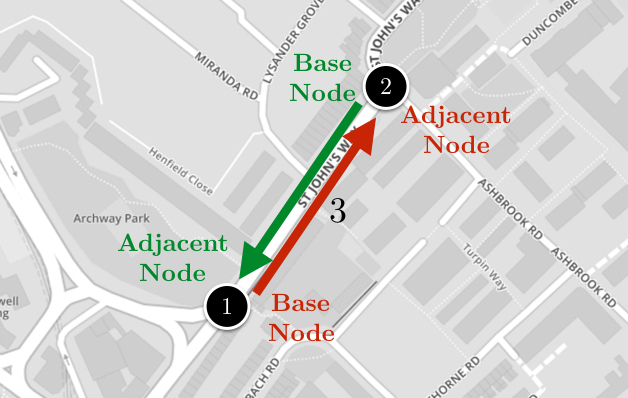
\includegraphics[width=\textwidth]{gh-edge-problem}
    \end{center}
    \caption{The problem with GraphHopper edges}\label{fig:gh-edge-problem}

    \vspace{0.6em}
    In the diagram above, we see two nodes with ID 1 and 2 joined by an edge
    with ID 3. Imagine we've performed two routing requests, one in red and
    one in green. Both routes go through edge 3, but in opposite directions.
    However, both edges will return true from the \texttt{isForward} method of
    \texttt{EdgeIteratorState}, despite going in opposite directions. Although
    GraphHopper knows that one of these is in reverse, the data is hidden from
    us.
    \end{greybox}
    \vspace{-2em}
\end{wrapfigure}

However, there is another challenge with regards to storing the data. When
parsing the ways, GraphHopper identifies the direction of the edge - each edge
can support moving either forward, reversed, or both. When a route is provided
by the routing engine, it is in the form of a list of
\texttt{EdgeIteratorState}s. The \texttt{EdgeIteratorState} class has been
designed to hide the `true' direction of the edge, instead switching which node
is the base node and which is the adjacent depending on the direction the
vehicle is travelling. The result of this is that every edge received from the
engine appears as a forward edge. For the cell model, we need to have two
separate directions for the roads, or vehicles going in opposite directions will
crash into each other and block the roads.

Figure \ref{fig:gh-edge-problem} illustrates why this is an issue. We are unable
to tell if we are travelling forwards or backwards based on the
\texttt{EdgeIteratorState} alone, as the ID is the same and the
\texttt{isForward} method returns true for both cases. This would not make it
impossible to identify if the forward or reverse cells should be used for the
vehicle. Initially, there was concern that a more complex solution than the
boolean arrays would be required - perhaps some kind of 2D mapping from pairs of
node IDs (or a base node and edge node) to a cell array. However, it is
important to note that we don't need to know if GraphHopper internally stores an
edge as forward or reverse so long as we are able to distinguish between the two
cases shown in Figure \ref{fig:gh-edge-problem}.

The technique we discovered to solve this uses the fact that the base node and
adjacent node returned by the edge changes depending on direction. As such, we
can define edges where the base node is greater than the adjacent node as
`forward' and edges where the base node is less than the adjacent node as
`backwards'. This allows us to reliably differentiate between the forward and
backwards cases, and save the vehicles from crashing into each other.

The \texttt{CellGraph} class handles the storage for the cells, providing
convenient getters and setters for edges at specific cells. It also
transparently handles the forward and reverse edges, storing two boolean arrays
(\texttt{boolean[][] cells} and \texttt{boolean[][] reverseCells}) and uses
whichever one is appropriate for the current EdgeIteratorState.

\subsubsection{Cell Size}\label{sec:cell-size}

One important question that must be answered is how many cells should be created
for each edge. According to the original paper, each cell should represent the
space a single vehicle takes up. In Europe, the average car is around 4.5 metres
long. Assuming that cars have at least a one metre gap between them suggests
that the cell size should be at least 5.5 metres. However, in the US the average car
length is 5 metres, suggesting 6 metres or more would be an appropriate cell
size. To accomodate these use cases and others, the size of cells is a
configurable parameter, allowing the users to pick an appropriate size for the
vehicles they are simulating.

\subsection{Vehicle and Cell Iterators}

\begin{figure}[h]
    \centering
    \includegraphics[scale=0.5,page=5,clip,trim=0 15cm 15cm 0]{architecture}
    \caption{The Nagel-Schreckenberg Model across edge boundaries.}\label{fig:nagel-multi}
\end{figure}

As we saw in Section \ref{sec:nagel}, one of the key parts of the
Nagel-Schreckenberg model requires vehicles to know how far they are from the
next vehicle. In \ref{fig:nagel-multi}, we see three vehicles - A, B, and C.
Vehicle A is 2 cells from B and 3 cells from C. A is soon to turn left onto the
edge with C, meaning it should not consider B as ahead of it.

However, each of these paths consists of multiple edges. We need a way of
treating lists of edges as a single continuous array of cells. This is a good
use case for the iterator pattern, providing us with an abstraction over the
underlying arrays.

The \texttt{VehicleIterator} class is responsible for storing and moving through
the vehicle's route. It stores the list of \texttt{EdgeIteratorState} objects and moves
to the next element each time its \texttt{next} method is called. It implements
the \texttt{EdgeIteratorState} API for full compatibility with GraphHopper. In
addition to the usual \texttt{EdgeIteratorState} methods, it can return the road
speed of an edge. It also removes the first and last elements from the list of
edges, as these are virtual edges created by GraphHopper that do not exist in
the \texttt{CellGraph}.

The \texttt{CellIterator} class stores the cell ID and the
\texttt{VehicleIterator}, meaning it can traverse across edge boundaries by
calling the \texttt{VehicleIterator}'s \texttt{next} method. It also has a
reference to the \texttt{CellGraph} so that it can return whether there is a
vehicle in the current cell.

\subsection{Vehicle Class}

The \texttt{Vehicle} class now has five core methods that are used for running the
simulation, rather than the single \texttt{calculateStep} function used before.
The \texttt{accelerationStep}, \texttt{slowStep}, \texttt{randomStep} and
\texttt{moveStep} all correspond to the four steps of the Nagel-Schreckenberg
algorithm, whilst the \texttt{updateLocation} method interpolates the cell
location into the edge geometry to find the vehicle's location.

The class also stores two core things that make the implementation possible.
The first is a \texttt{VehicleIterator} named \texttt{route} containing the
list of edges each vehicle will take, as well as its current edge. The second is
the current cell ID the vehicle is on. By duplicating the
\texttt{VehicleIterator} and passing it to a new \texttt{CellIterator}, the
vehicle can find out if it is able to accelerate or must slow down - even if the
vehicle in front is multiple edges ahead.

\begin{minipage}{\linewidth}
\begin{lstlisting}[caption={The \texttt{slowStep} implementation making use of the CellIterator},
                    label=lst:slowStep, numbers=left]
public void slowStep()
{
    int j = 0;
    CellIterator c = new CellIterator(new VehicleIterator(route), cg, cellId);

    while (!c.next() && j <= v)
        j++;

    if (j <= v)
        v = j;
}
\end{lstlisting}
\end{minipage}

Listing \ref{lst:slowStep} shows how the CellIterator and VehicleIterator work
in conjunction to implement the slow step of the Nagel-Schreckenberg method.
The variable \texttt{j} represents the distance to the next vehicle, whilst
\texttt{v} is the vehicle's current velocity. Line 4 shows the initialisation of
the CellIterator - note that \texttt{route} is a VehicleIterator being created
with a copy constructor, meaning that the current location of the vehicle will
not be changed from this CellIterator.

\subsection{Results and Evaluation}

At this point, the system was capable of simulating any number of vehicles with
realistic traffic flow behaviour. However, there were still many key performance
improvements that needed to occur before the system would be ready for
algorithm development.

\begin{itemize}
    \item The back end still waits one second per iteration.
    \item The back end architecture does not allow for vehicles with different
        behaviour.
    \item The back end does not make optimal use of the multiple threads and
        cores that modern computers have available to them.
    \item The front end has graphical glitches and poor performance when
        showing more than 16,000 vehicles.
    \item Metrics for later data analysis are not recorded.
    \item Additional vehicles can not be added to the simulation once it has
        started.
    \item The simulation cannot be paused or resumed.
\end{itemize}

\section{Performance and Architecture Improvements}

There were two core goals for the system at this stage. Firstly, improve
performance such that at least 64,000 vehicles can be simulated and secondly,
modify the architecture of the system to support multiple vehicle types with the
ability to have different vehicle types running side by side.

\subsection{Front-end Performance}

Before this stage of the project, the front end had many performance issues.
With enough vehicles, the entire page would become slow to respond and update.
Even with the one second delay, it would sometimes fail to update before
receiving the next set of data.

\begin{figure}[h]
\centering
\begin{subfigure}[b]{0.4\textwidth}
    \centering
    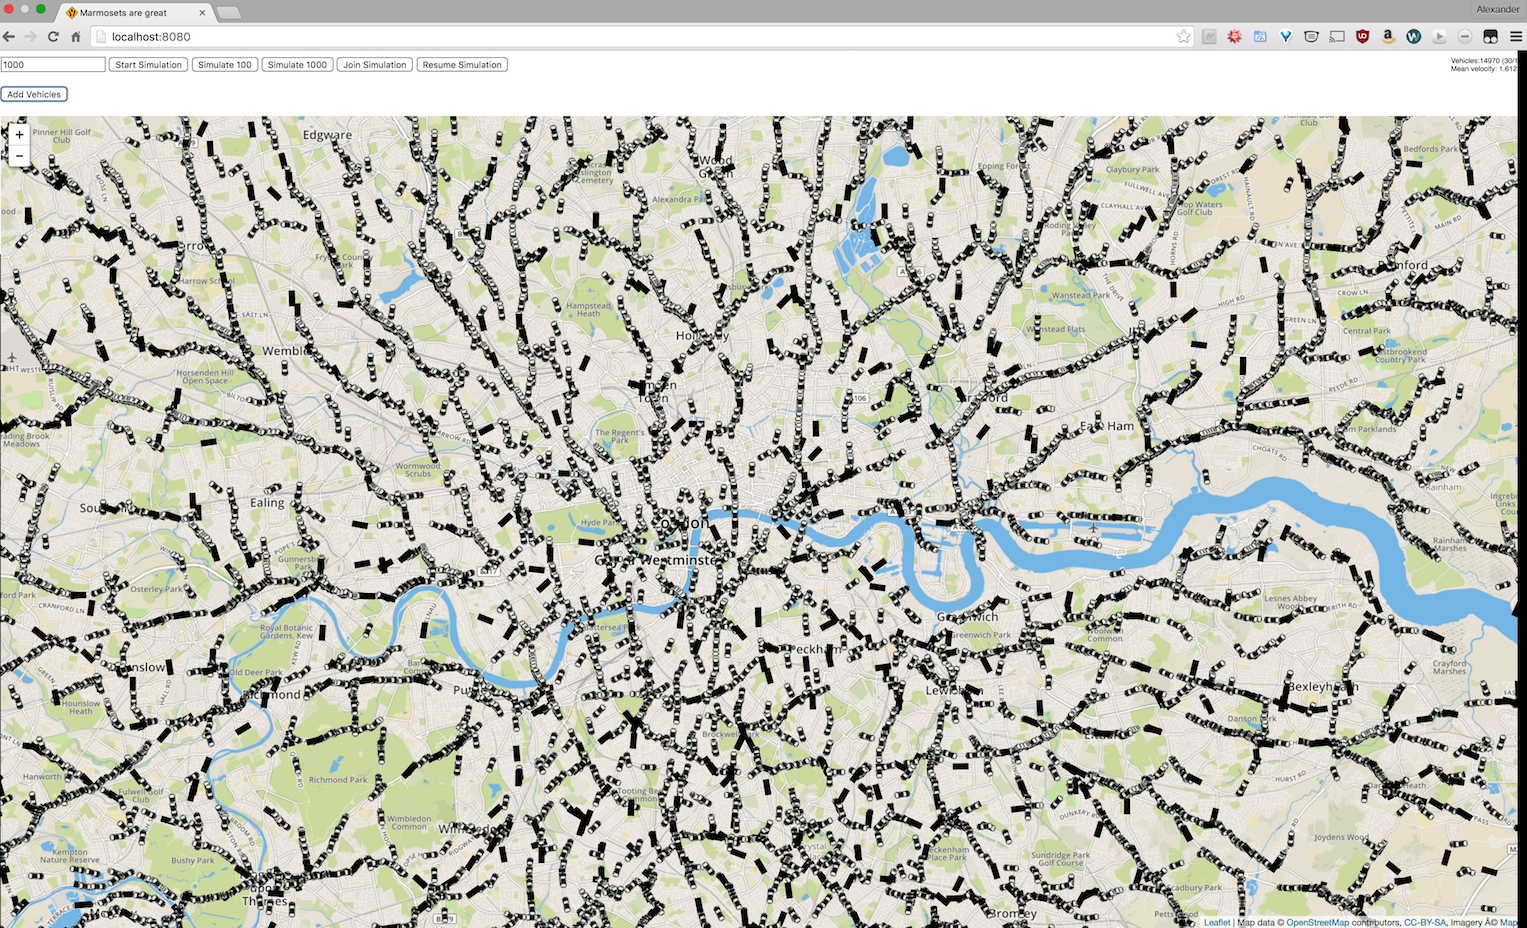
\includegraphics[height=9em]{glitches-car}
    \caption{Vehicles showing up as black squares rather than image icons.}\label{fig:glitches-car}
\end{subfigure}
\hspace{3em}
\begin{subfigure}[b]{0.4\textwidth}
    \centering
    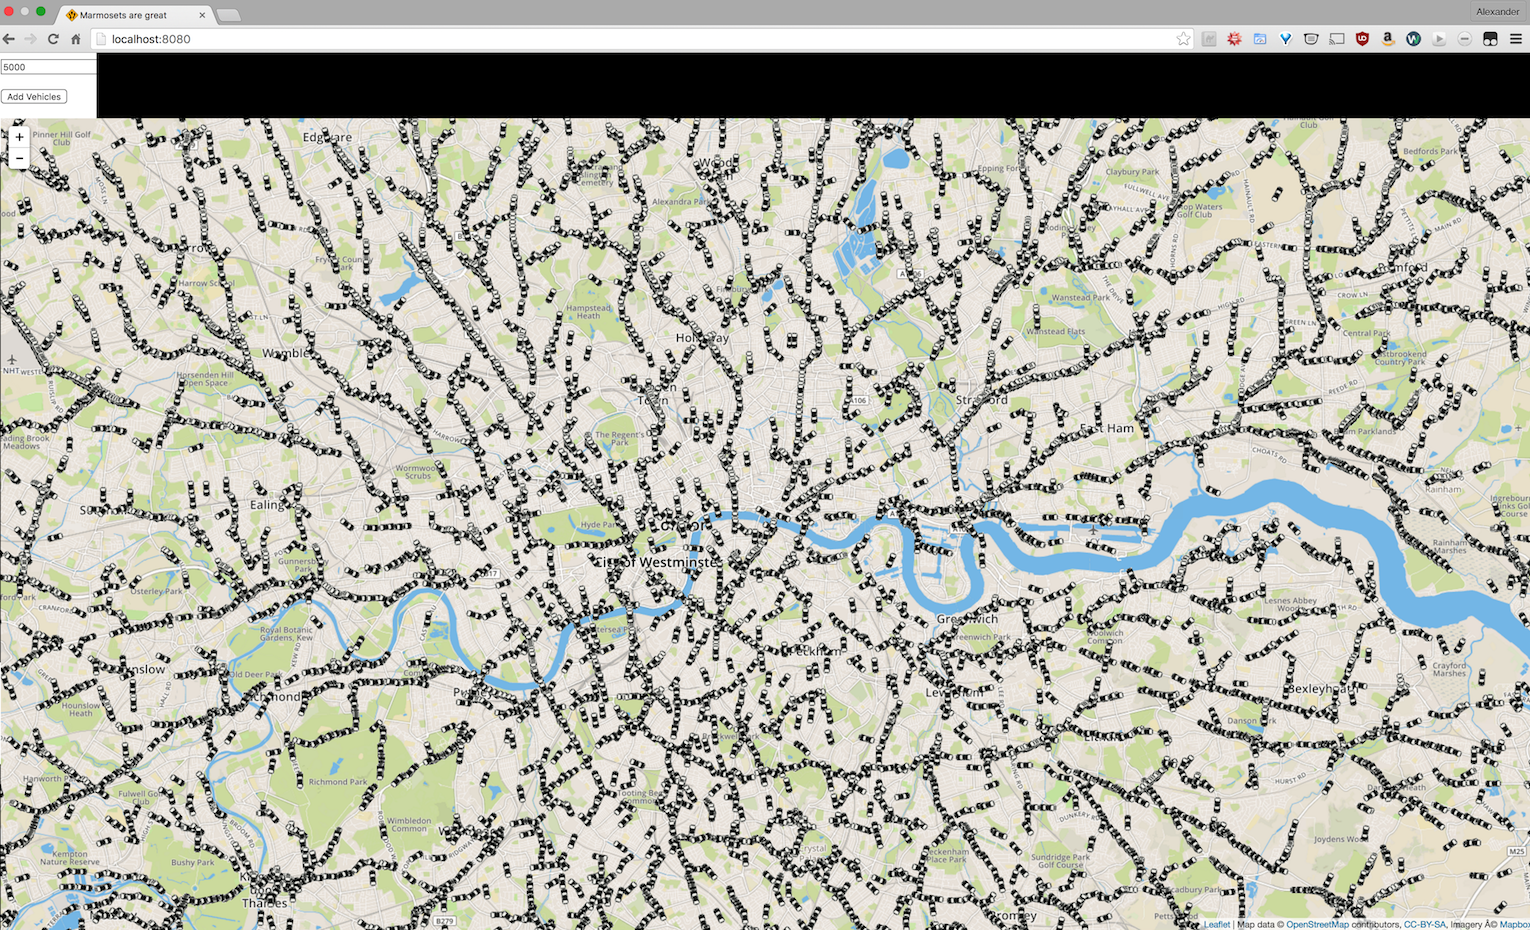
\includegraphics[height=9em]{glitches-chrome}
    \caption{Large black blocks showing over parts of the screen.}\label{fig:glitches-chrome}
\end{subfigure}
\caption{Graphical glitches caused by displaying more than 16,000 images.}
\end{figure}

\subsubsection{Marker Rendering}

Initially, the Leaflet.AnimatedMarker library was used to make it appear as
though the vehicles were driving around the map in real-time. However, this had a
huge performance cost, and as such had to be disabled.

Additionally, the vehicle image used was reasonably large and in colour.
Creating a much smaller vehicle image (from 15KB to 1KB) improved performance a
little, but did not raise the 16,000 vehicle limitation.

One of the core issues with the existing implementation was the use of
\texttt{img} tags for displaying the vehicles. As each HTML tag is a full blown
element in the DOM, there is a reasonably high performance cost associated with
their use. There are two main alternatives for showing graphics in the browser -
SVG and the HTML5 Canvas API.

\begin{wrapfigure}{l}{0.35\textwidth}
    \vspace{-1em}
    \begin{greybox}
        \centering
        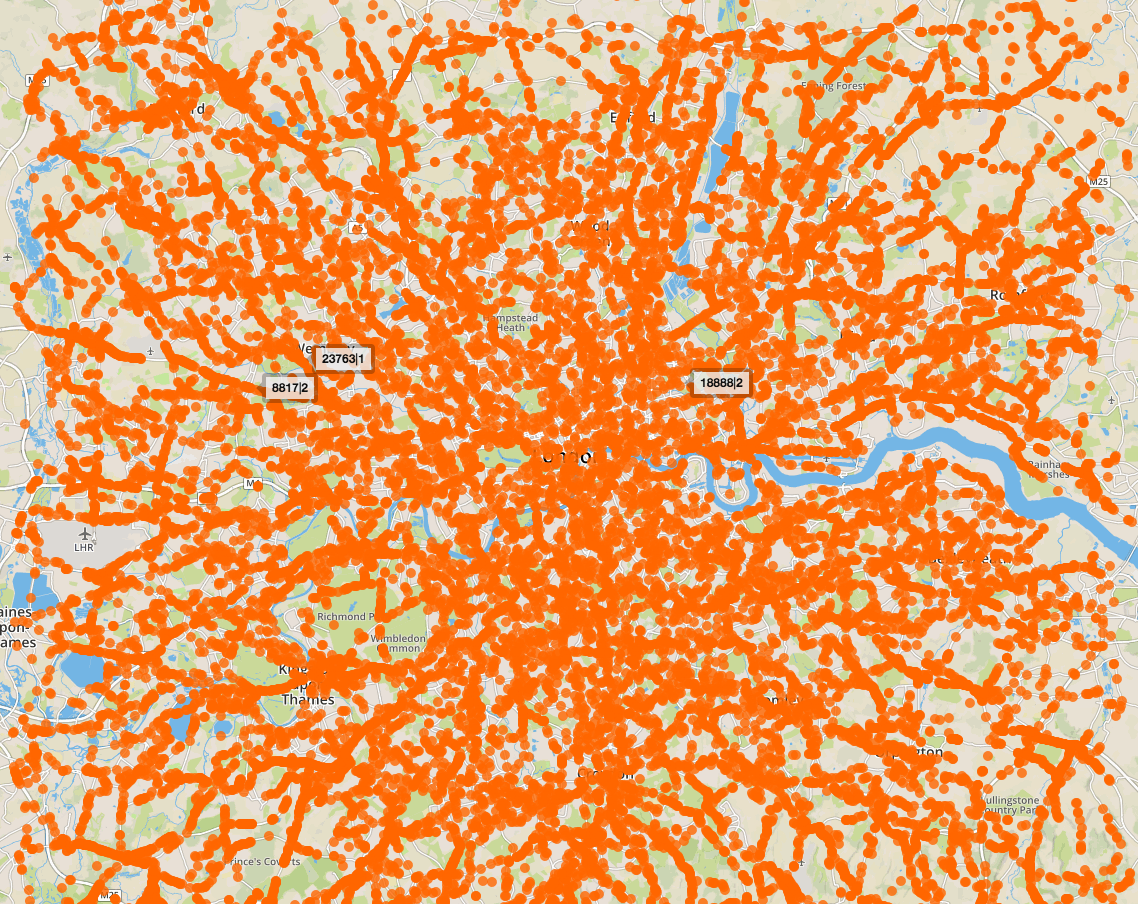
\includegraphics[width=\textwidth]{orange-markers}
        \caption{SVG Rendered orange markers showing 30,000 vehicles}\label{fig:orange-markers}
    \end{greybox}
    \vspace{-3em}
\end{wrapfigure}

Unlike the \texttt{img} tag, the Canvas API is designed for drawing and other
graphical purposes. Instead of one tag per vehicle, A single \texttt{<canvas>}
element would be able to render every vehicle. We had been concerned that there
would be major challenges in extending the Leaflet Marker class to use an
entirely different way of showing markers, but thankfully Leaflet provided the
location to display the markers in pixels to \texttt{Marker} subclasses. Using
Canvas offered drastically improved performance with seemingly no upper limit on
how many vehicles the front end could display with no glitches.

However, there were a few downsides to using Canvas. Firstly, the map correctly
re-rendered all the markers when zooming in and out, but did not update the
markers when panning the map. Attempts at fixing this issue were unsuccessful.
Additionally, the \texttt{img} tags were able to support a popup when mousing
over a vehicle that showed its current speed and ID, which was useful for
debugging.  This would have to be implemented by hand to be supported with
Canvas - manually detecting the current mouse position, checking which vehicle
it was hovering over and then drawing a custom popup on top of the view.

Instead, we experimented with SVG, an XML based web API for vector graphics. One
key advantage is that Leaflet has built in support for drawing certain types of
SVG elements. The static image marker could simply be replaced with a
\texttt{CircleMarker}, which used the same API as the Marker and AnimatedMarker,
but instead shows a circle with customisable radius and colour.

SVG combined the performance of Canvas (rendering 64,000 vehicles whilst
remaining responsive) and the interactivity of img tags (panning around the map
worked flawlessly, and popups worked with no additional work). The only downside
was that a circle is shown instead of a vehicle icon, meaning it is not possible
to rotate the shape to indicate which direction the vehicles are travelling.
This is a minor price to pay for the performance improvements, so the decision
was made to use SVG for the front end moving forwards - the result can be seen
in Figure \ref{fig:orange-markers}.

\subsubsection{WebSocket Data Format}

The back end initially just sent down data in string format - for example a
vehicle with ID 10067 could have a string of
\textit{10067|51.5306611887|0.1609468558|1}. This format has a number of
issuses. Firstly, there is limited precision for the values, as they must be
truncated to a certain number of decimal places.  Secondly, the format is text
based, meaning there is a much larger overhead of space compared to storing the
values numerically. Finally, it takes additional time to convert the data into a
string only to parse it back into numerical values on both the front end and
back end.

The string data required for updating the locations of 1000 vehicles takes 33Kb.
Encoding this as raw binary data requires 4 bytes for the vehicle ID and speed
each and 8 bytes for each of the latitude and longitude, requiring 24 bytes per
vehicle and hence 24Kb for the total transfer.  This is not only smaller, but
also comes with a performance and accuracy improvement as well.

Thankfully, the WebSocket protocol supports the sending of binary data, which
can then be efficiently processed by the front end using the DataView APIs. On
the back end, we create a single reusable BinaryBuffer object and pass it to the
Vehicles, which add their data into a specific offset. This is significantly
more efficient than the string based method, although the change is primarily
for improving network and front end performance.

\subsection{Back end Performance}

\subsubsection{Removing the time-lock}

The most necessary change was removing the added delay for the timestep from the
Marmoset class. Instead of sending the data every second, the socket server
waits for a `next' message from the front end to start processing the next
timestep. It then sends the data and continues to wait for the command to
continue.

This drastically improved the speed of the system. For low numbers of vehicles,
each timestep takes little more than a few milliseconds on both the front and
back end. 1000 iterations with 1000 vehicles used to take at least 16 minutes -
after making this change it took just 50 seconds.

Additionally, this allowed much larger numbers of vehicles to be simulated and
visualised at the same time - the back end will only send data to the front end
once it has rendered the previous set of changes.

This also made it easier to add the ability to pause the simulation - by simply
ceasing to send the \texttt{next} message, the back end does no further work,
leaving the user able to explore the current state of the simulation in the
browser.

\subsubsection{Exploiting Parallelism}

Initial versions of the system simply did all their work on a single thread.
There were a number of places were task-level parallelism made it easy to add
more threads and cores to the system to improve performance.

\begin{minipage}{\linewidth}
\begin{lstlisting}[caption={The single-threaded \texttt{timestep} function},
    label=lst:timestep]
public void timestep()
{
    vehicles.stream().forEach(Vehicle::accelerationStep);
    vehicles.stream().forEach(Vehicle::slowStep);
    vehicles.stream().forEach(Vehicle::randomStep);
    vehicles.stream().forEach(Vehicle::moveStep);
    vehicles.stream().forEach(Vehicle::updateLocation);

    vehicles.stream().filter(v -> !v.isFinished()).collect(Collectors.toList());
}
\end{lstlisting}
\end{minipage}

In Listing \ref{lst:timestep} we can see the use of the Java 8 Stream API to run
the Nagel-Schreckenberg functions on each vehicle. One of the core features of
the API is built-in support for concurrency. By replacing the calls to
\texttt{stream()} with \texttt{parallelStream()}, Java will automatically split
the computation over multiple threads, whilst ensuring that all processes have
completed when the next line is executed. The \texttt{vehicles} list was
replaced with a synchronised list to ensure that removing finished vehicles from
the collection was still thread-safe.

When adding new vehicles to the simulation, their initialisation uses
GraphHopper to find the route to their destination. This takes orders of
magnitude longer than the timesteps themselves, and as GraphHopper routing
requests are thread-safe is an easy way to further improve performance.

\subsection{Architecture Improvements}

One of the issues with the system at this point was the lack of support for
multiple vehicle types - although there is a \texttt{Vehicle} class that could
have been be subclassed, it was not easy to modify its behaviour without having
to rewrite large portions of the code.  As such, this part of the system was
refactored to improve the architecture of the system.

\subsubsection{Vehicle Refactoring}

\begin{figure}[h]
    \centering
    \includegraphics[scale=0.6,page=6,clip,trim=0 11cm 8cm 0]{architecture}
    \caption{The Vehicle and VehicleIterator class structure}\label{fig:veh-arch}
\end{figure}

Following the refactor, the \texttt{Vehicle} and \texttt{VehicleIterator} are
now interfaces of the public methods originally implemented in the Vehicle
class.  \texttt{BaseVehicle} and \texttt{BaseVehicleIterator} are abstract
classes that implement most of the boilerplate functionality.
\texttt{BaseVehicle} holds the implementation of the Nagel-Schreckenberg model,
with routing behaviour defined by the \texttt{VehicleIterator}. A subclass of
\texttt{BaseVehicle} must implement only a single method -
\texttt{getVehicleIterator()}, which creates a \texttt{VehicleIterator} of the
correct type and with the right routing information.

For the standard routing algorithm, new \texttt{DijkstraVehicle} and
\texttt{DijkstraVehicleIterator} classes have been created. As a way of
verifying that multiple vehicle types are possible, a \texttt{RandomVehicle} and
corresponding \texttt{RandomVehicleIterator} that simply drive around at random
with no overarching behaviour were implemented.

\subsection{Metric calculations}

The initial engine only allowed for viewing the results of an algorithm by
looking at the visualisation - it is also important to be able to perform
offline analysis of the data.

Brief calculations showed that storing the full movement of 64,000 vehicles
could take up to 10GB of storage, suggesting that it was better to calculate
metrics at each timestep and store those instead. There are three main types of
metric - vehicle, route and network metrics.

\subsubsection{Vehicle Metrics}

As their name suggests, vehicle metrics provide information about the state of
one or more vehicles. They can be calculated at any time, so can be recorded and
stored on each iteration. Vehicle metrics are the easiest way of getting a sense
of the overall behaviour of the system at a given point in time.

With the goal of understanding the levels of congestion, two main vehicle
metrics were tracked: the number of vehicles not moving at the maximum road
speed and the number of vehicles that slowed down due to a vehicle in front of
them.

A new inner \texttt{Metric} class was added to \texttt{MarmosetHopper}, with
simple data properties storing the average values for the two metrics mentioned
above, as well as the total number of vehicles and the average speed (in cells
per second) of the vehicles. The \texttt{toString} method has also been
overridden to print the data in CSV format, with a separate static method to
return the header for the CSV file.

\subsubsection{Route Metrics}

We can also better understand congestion by looking at the length of time it
takes for a vehicle to reach its destination. Inside the simulation engine, the
\texttt{Vehicle} class simply tracks the number of iterations it has travelled
before reaching its destination.

The GraphHopper \texttt{GHResponse} class stores the length of time a route is
expected to take, which can be compared to the actual journey time. Although it
does not include a realistic model of vehicle behaviour (so does not truly
represent the correct time a journey would take, even on empty roads), the
difference between expected and actual time is another metric that can be used
to compare different vehicle behaviours.

Route metrics can only be recorded once the vehicle has reached its destination
rather than whilst it's travelling. As such, a \texttt{printMetrics} function
was added to \texttt{BaseVehicle} with an implementation in
\texttt{DijkstraVehicle} that prints the expected time from GraphHopper and the
actual number of iterations the vehicle took to reach its destination.

These metrics are output into a file named after the ID of the vehicle in
question - each vehicle has its own file, meaning there is no need for
centralised management of writing to disk.

\subsubsection{Network Metrics}

\begin{wrapfigure}{r}{0.4\textwidth}
    \vspace{-1em}
    \begin{greybox}
        \centering
        \includegraphics[width=\textwidth]{dijkstra-15k-wide}
        \caption{Post-simulation analysis of the 9,000th iteration of 15,000 vehicles}\label{fig:offline-network}
    \end{greybox}
    \vspace{-3em}
\end{wrapfigure}

Network metrics provide information about the roads themselves and how congested
or occupied they are. Instead of providing numerical data for every edge (which
provides very little information given how few cells/vehicles the average edge
has), a visual approach was used, simply retaining the full set of vehicle
positions and speed every 1000 iterations.

The code previously used to convert the Vehicle objects into strings was
re-purposed, with the output placed into an iteration file. This means that the
data is human readable and easy to parse. On the front end, an input box with
basic parsing code was added to allow the data to be explored interactively
after the simulation has finished, as can be seen in Figure
\ref{fig:offline-network}.

\subsection{Event System}

Although the refactors mentioned above do allow for a large amount of
flexibility, using new vehicle classes (or adding new behaviour on each
timestep) required modifying the \texttt{MarmosetHopper} class directly. Using
an events system enables users of the engine to add code and functionality
during key points of the program's execution without directly modifying the
engine.  Instead, users can call a \texttt{listenTo} method with a callback
function that is executed when the event is triggered.

Event triggers were added in key locations so that these features would be
useful. For example, an event is triggered at the start and end of each
timestep, at the beginning and end of initialisation and when a new vehicle is
added.

\subsection{Offline Simulation}

With the addition of metrics, it became clear that it would be useful to be able
to run a simulation in the background and analyse the data later. One use case
would be understanding how long it takes all vehicles to reach their
destinations; another is for analysing very high density networks where it may
not be desirable to view the data on screen in real-time due to the added
performance cost.

A command line flag (\texttt{-{}-file}) was added with an argument for the
number of vehicles to be simulated as well as a custom name. The simulation
creates a folder for the metrics including the number of vehicles, a Unix
timestamp, and the chosen name, allowing it to be uniquely identified.

However, the offline simulation appeared to be running slower than hoped given
it was not constrained by the browser rendering. The VisualVM Java profiler was
used to identify potential performance improvements whilst simulating.  Far more
time was spent in the \texttt{updateLocation} step than expected - and given
that the physical location is only used for display and not internal routing, a
function parameter was added to disable the location updates when simulating
offline.  Instead, the location is only updated when required (e.g for
outputting the locations every 1000 iterations).

\begin{figure}[h]
    \centering
    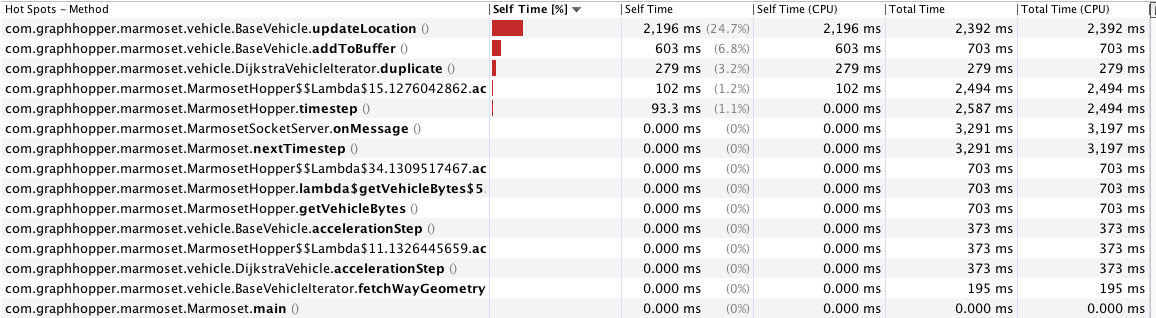
\includegraphics[width=0.9\textwidth,clip,trim=0 7cm 0 0]{visualvm-profile}
    \caption{VisualVM Profile of the most time consuming functions}\label{fig:visualvm}
\end{figure}

Removing the location updates had a drastic improvement to offline performance,
reducing a simulation from TIME A to TIME B. Simulations with large numbers of
vehicles could now be simulated to completion in a reasonably short amount of
time.

\section{Algorithm Design and Implementation}

As a way of exploring the capability of the simulation engine, a multi-vehicle
routing algorithm was designed, implemented and tested.

\subsection{Algorithm Design}\label{sec:algo}

We chose to design a V2I algorithm, as there would be a substantial amount of
additional code required to simulate realistic V2V communication. It is also
beneficial that V2I simulation can apply to both high and low density situations
as it is not limited by the distance to the nearest vehicle. Furthermore, V2I
algorithms that rely only on mobile connections are able to work with both human
drivers and self-driving cars, unlike V2V algorithms that would require all
vehicles to have new hardware and software.  Instead, access to a central system
that knew the location and planned destination of every vehicle in a city is
assumed. The algorithm then provides routes for each vehicle in the system.

The initial design of the Marmoset algorithm is described below. It is
important to note that this is not the final algorithm - the goal was to find a
technique that could potentially be effective and then optimise, improve and
understand it using the simulation engine.

\subsubsection{Vehicle Behaviour}

Individual vehicles make their current route and position available to
the central system at all times. The vehicles request routes from the system and
then follow them directly. A vehicle requests a new route after a random
interval (based on a predetermined parameter).

\subsubsection{Central System Behaviour}

The central system stores the number of vehicles that have been told to route
along each edge, called the Expected Map. It is initialised with zero values for
all edges on start-up.

\begin{wrapfigure}{r}{0.4\textwidth}
    \vspace{-1em}
    \begin{greybox}
        \centering
        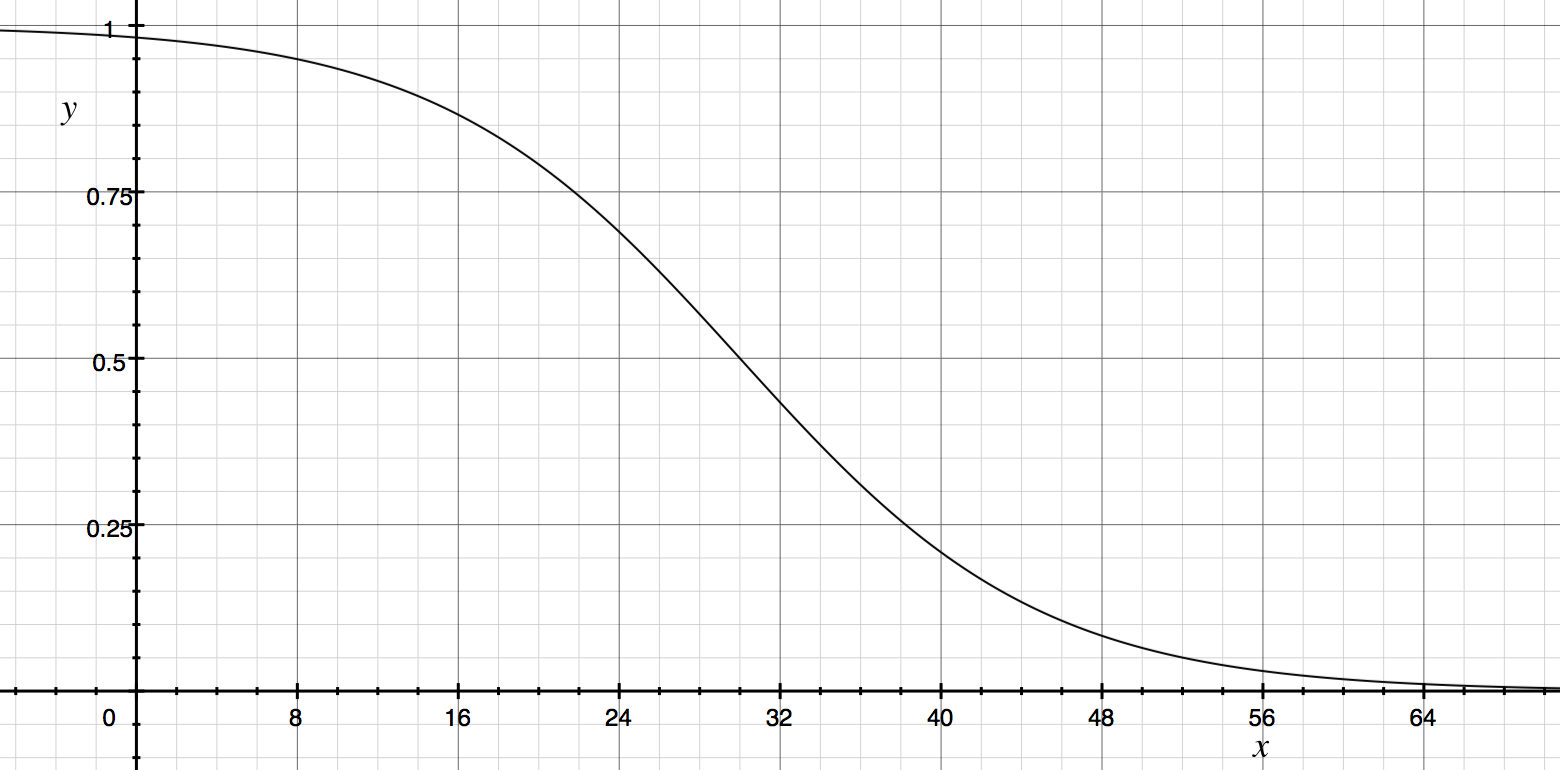
\includegraphics[width=\textwidth]{congestion-crap}
        \caption{The initial choice of congestion function.}\label{fig:cong-crappy}
    \end{greybox}
    \vspace{-3em}
\end{wrapfigure}

At a fixed interval, the system updates the Expected Map by multiplying every
edge by a damping factor that is less than 1. It then adds the edges in each
vehicle's current route to the Expected Map.

When a route is requested, the data from the Expected Map is used in conjunction
with a congestion function to modify the weight of edges based on their expected
density. This will return a route that avoids high-congestion roads, which will
be reflected in the Expected Map upon its next update.

The graphs in Figures \ref{fig:congestion-graph} and \ref{fig:congestion-graph-2} were similar in nature to a
sigmoid function such as $\tanh$, so this was used as the foundation for the
congestion function. Adjusting the scale and position of the function led to the
graph shown in Figure \ref{fig:cong-crappy}, $\displaystyle v(x) = \frac{\tanh(2-\frac{x}{15})+1}{2}$.

\subsubsection{Design Justification}

\begin{wrapfigure}{r}{0.5\textwidth}
    \vspace{-1em}
    \begin{greybox}
        \centering
        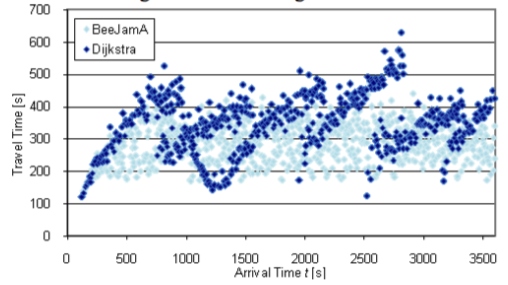
\includegraphics[width=\textwidth]{beejama}
        \caption{Oscillation of travel time when using Dijkstra's algorithm with traffic information.}\label{fig:bjam-dijkstra}
    \end{greybox}
    \vspace{-2em}
\end{wrapfigure}

The goal of the Expected Map is to help vehicles avoid roads that are likely to
have high levels of traffic. However, a na\"{i}ve approach to this would result
in oscillatory behaviour between optimal and sub-optimal routes, as can be seen
in Figure \ref{fig:bjam-dijkstra}. As such, the Expected Map is retained for
further requests. The first step of updating the Expected Map multiplies each
value by the damping factor. This is to stop the system from having too much of
a memory (and hence over-penalising roads that will have many vehicles on them).
This factor can be adjusted to define how much memory the system will have of
the vehicles' routes.

Furthermore, the system can handle the expectation that most routes will
change at some point whilst the vehicle is on the road. The random rerouting was
chosen to ensure that the busy areas will not be avoided by all vehicles once the
Expected Map has shown that they will be busy. If every vehicle was rerouted
simultaneously, the vehicles would completely avoid the busy roads and hence
fail to use the network capacity available to them.

\subsection{Implementation}

The implementation of this algorithm made use of the new event system and
required the subclassing of two GraphHopper types. A central self-driving vehicle
controller class was also created that manages the behaviour of all the
vehicles.

In keeping with the new system architecture, \texttt{SelfDrivingVehicle} and
\texttt{SelfDrivingVehicleIterator} classes were created. The SelfDrivingVehicle
class is similar to the DijkstraVehicle, but offers new methods for
recalculating the route using the expected weighting. The
SelfDrivingVehicleIterator is a subclass of the DijkstraVehicleIterator, but
adds a simple method for replacing the list of edges once a new list has been
calculated by the SelfDrivingVehicle class.

The Expected Map was implemented by creating a GraphHopper weighting class,
\texttt{ExpectedWeighting} (see Section \ref{sec:gh-weighting}). It stores an
array of floating point values representing the Expected Map (\texttt{double
expectedMap[]}) and has an \texttt{updateExpectedMap} method that applies the
damping factor and adds vehicle routes to the map. The weighting's
\texttt{calcWeight} method uses the curve described in the previous section to
return a weighting for an edge given the value in the Expected Map and the speed
of the road.

This is all orchestrated by the \texttt{MultiSDVController} class, which stores
a list of all \texttt{SelfDrivingVehicles}. It subscribes to the ``vehicle:add'' event
to create its own list of vehicles, as well as the ``timestep:end'' event for
triggering the re-routing and updating of the Expected Map.

The \texttt{MultiSDVController} was also optimised to exploit parallelism for the
re-routing operations. As it was not a use case suited to the parallel stream
API, an \texttt{ExecutorService} is used to manage and shutdown the threads for
routing as required.

\subsection{Testing}

\subsubsection{Algorithmic Adjustments}

Initial tests of the algorithm showed poor performance and many failed routes.
Use of the visualisation aspect of the routing engine was crucial in identifying
the causes of this.

The first issue was caused by the congestion function. As the expected value for
each edge represents how many vehicles will ever drive on that road (rather than
at one time), the numbers are usually much larger than the number of vehicles
that would be on the road at any given time. As such, the values returned by the
congestion function were often very close to (or sometimes exactly) zero. The
end result of this was that after a few recalculations of the Expected Map, any
popular edge was completly removed from the graph, and hence connections to
high-congestion areas of the map were removed entirely.

It is not entirely undesirable to remove roads high congestion roads from the
graph. However, this would require perfect knowledge that a given road will be
blocked - due to the non-deterministic nature of the vehicles (caused by the
re-routing opreation), this cannot be guaranteed and hence edge removal is not
appropriate for the routing algorithm. In response to this discovery, the
congestion function was modified to have a lower bound of 25\% of the original
road speed, using the same curve shape as before. The function used can be seen
in Figure \ref{fig:final-cong-func}.

The other issue was that many roads near a vehicle's destination would have very
high values in the Expected Map, creating routes that avoided moving towards the
destination. This was partly due to the fact that the vehicle was attempting to
avoid road penalties created by its own routes. This was fixed by using a
progress function - instead of simply incrementing the value at the edge by one,
it is incremented by a value determined from the progress function. The progress
function takes in a percentage - the edges percentage in the route - and outputs
a value that decreases as we reach the vehicle's destination. The justification
for this behaviour is that a vehicle is much more likely to visit an edge nearer
to it than further away, as it has a higher probability of having re-routed by
then. The progress function can be seen in Figure \ref{fig:final-prog-func}.

Additionally, it was found that random routing did not have the desired effect -
many vehicles never adjusted their routes, whilst others re-routed as many as
seven times during a single simulation. This was problematic as the end result
was too many vehicles remaining on the highly congested routes, even if the
Expected Map showed that they should be avoided.

\subsubsection{Parameter Adjustments}\label{sec:parms}

The algorithm offers five core parameters that can be adjusted, listed below.

\begin{figure}[h]
    \centering
    \begin{subfigure}[b]{0.45\textwidth}
        \centering
        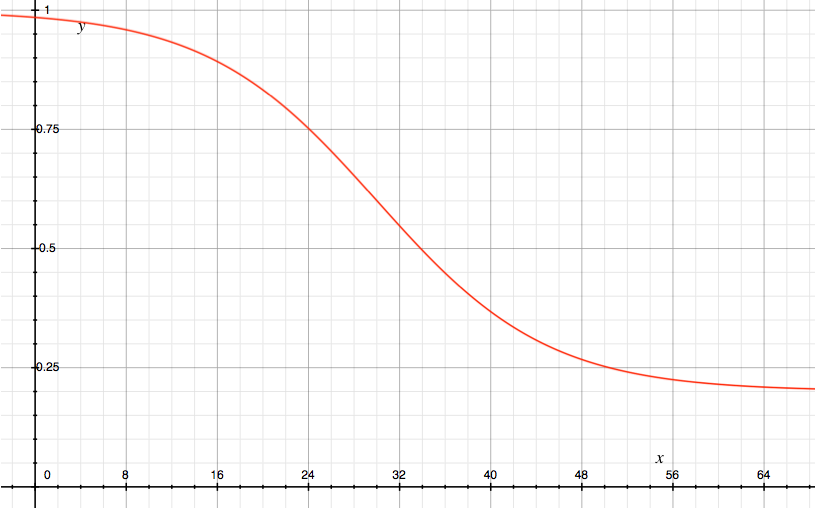
\includegraphics[height=10em]{congestion-function}
    \caption{The congestion function.}\label{fig:final-cong-func}

    $\displaystyle v(x) = \frac{\tanh(2-\frac{x}{15})+1.5}{2.5}$
    \end{subfigure}
    \begin{subfigure}[b]{0.45\textwidth}
        \centering
        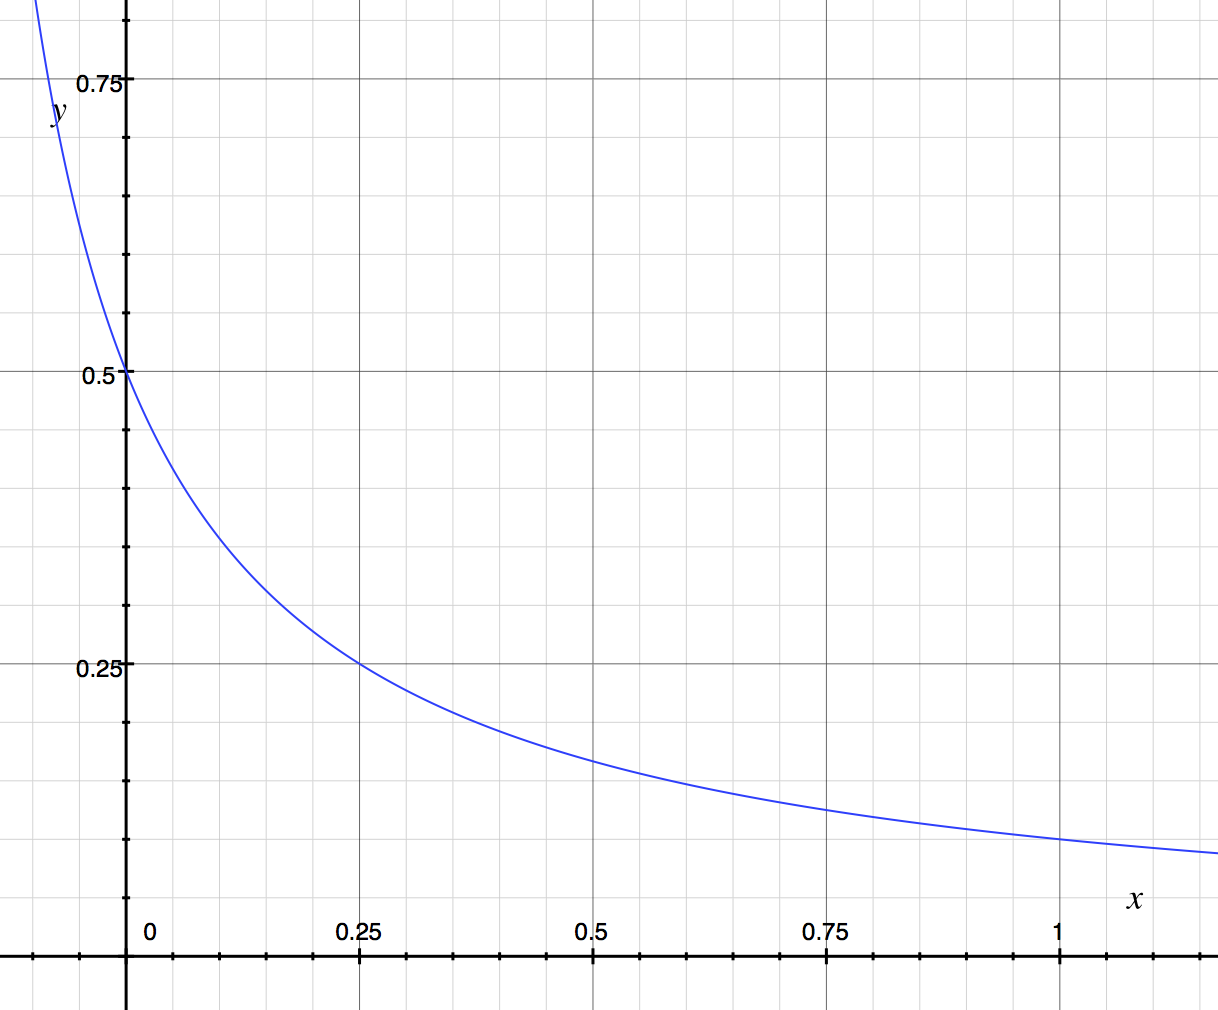
\includegraphics[height=10em,clip,trim=1cm 5mm 0 6cm]{progress-function}
        \caption{The progress function.}\label{fig:final-prog-func}

        $\displaystyle f(x) = \frac{1}{8x + 2}$
    \end{subfigure}
\end{figure}

\begin{itemize}
    \item \textbf{Congestion function} - can be modified to reduce penalties overall,
        behave differently for different types of road, or have a longer or shorter
        tail.
    \item \textbf{Progress function} - can be modified to decrease or increase
        values on nodes further away.
    \item \textbf{Re-routing percentage} - can be modified to change how quickly the
        vehicles react to high-congestion areas.
    \item \textbf{Damping factor} - can be modified to change the memory of
        the Expected Map.
    \item \textbf{Expected map update frequency} - can be modified to change how
        fast the system reacts to vehicles changing their routes.
\end{itemize}

After a few minor experiments, the congestion function shown in Figure
\ref{fig:final-cong-func} was used for testing the algorithm, as it penalised
busy roads without causing overly long routes for most vehicles. Likewise, the
progress function in Figure \ref{fig:final-prog-func} was chosen to ensure that
central roads would not be repeatedly penalised and cause undesirable results.

The damping factor was initially chosen as 0.6, meaning that the edges kept 60\%
of their value when the Expected Map was updated. This proved to be too high,
causing extended travel times when simulating. After brief experimentation, a
lower value of 0.2 was used and found to be more effective.

The re-route percentage has an impact on both the behaviour of the vehicles and
the performance of the engine - the more vehicles it has to reroute on each
iteration, the longer the simulation takes overall. With a re-route percentage
of 0.1\%, simulating 64,000 vehicles requires 640 re-routing operations at each
timestep. On a many-core server, this took approximately one second per
iteration. This was a slow but acceptable compromise, as the simulation could be
left to run overnight and analysed after the fact using the metric data.
Furthermore, the speed of each iteration increases as more vehicles reach their
destination, due to the number of vehicles to re-reoute decreasing.

There are also a number of parameters that must be selected for the simulation
engine itself.

\begin{itemize}
    \item \textbf{Cell size} - can increase or decrease number of vehicles each
        road can have, also affects max speed of roads.
    \item \textbf{Slow probability} - modifying the probablity a vehicle slows
        down (as described by the Nagel-Schreckenberg algorithm) can be adjusted
        to simulated different types of driving behaviour.
    \item \textbf{Vehicle destinations} - start and end location of vehicles can
        be adjusted to better model/understand traffic flow under different
        conditions.
\end{itemize}

Due to the increasing size of European vehicles and to account for
larger vehicles like trucks or vans, 6.5 metres was chosen to be the size of
cells in simulation. Brief tests showed that this had a negligible impact on
the overall performance of the algorthm, having the same effect as minorly
reducing the vehicle density.

For the slow probability, a value of 0.4 was chosen based on research in
\cite{nagel-detail}. There are various valid values for the probability, ranging
from 0 to around 0.5. If the value is too low, the model does not simulate
traffic jams, whilst a value too high would fail to match reality.

A simple model of rush hour was created for the purpose of evaluating the
algorithms. Each vehicle is given a random location and destination within
London. The starting location is randomly distributed within the entirely of
London, appproximately bounded by the M25. The destination is randomly
distributed across the centre of London only, roughly covering Zone 1. Each
algorithm was simulated with 10,000 to 80,000 vehicles in increments of 10,000,
with the goal of understanding how traffic flows differently within each
algorithm.

\subsubsection{Evaluation}

This section will discuss testing methodology, with the results of the algorithm
and the overall performance of simulation engine discussed in Chapter
\ref{chap:evaluation} below.

Evaluating how two different routing algorithms would behave in any situation is
a challenging task with a near unlimited scope, particularly with complex
algorithms relying on the interactions between tens or even hundreds of
thousands of separate entities. As such, the scope of the evaluation has been
limited to one key scenario in a particular location. London has been chosen for
the location, due to the author's familiarity with its roads and expected
congestion. The tests will be a simple simulation of rush hour, when 64,000
vehicles~\cite{tfl} travel into the city centre.  Congestion during this period
of time is often at its worse, in spite of attempts by TfL to reduce travel at
peak times.

Tests will focus on a single parameter at a time. The tests for different cell
sizes and vehicle density will be run with both the Marmoset and Dijkstra
algorithms, whilst the tests for the Marmoset progress and congenstion functions
will only be compared to other Marmoset tests.

Interestingly, when testing the rush hour simulation using Dijkstra's algorithm
with 30,000 vehicles or more, unexpected behaviour was discovered. Namely, the
simulation would not terminate due to congestion in a closed loop around
Elephant \& Castle roundabout. All vehicles would slow to a halt along a fixed
number of fully congested roads, as can be seen in Figure \ref{fig:dijkstra-wtf}.

As such, new termination conditions were added. If every vehicle has slowed due
to a vehicle ahead, is not at the road's maximum speed, and the average speed of
the vehicles is near zero, the simulation terminates early. For 60,000 vehicles,
early terminaton happens after approximately 21,000 iterations - with 30,000
vehicles this state is reached in around 12,000 iterations, whilst 20,000
vehicles terminates completely (with 0 vehicles yet to reach their destination)
in a little over 9,000 iterations.

% -----------------------------------------------------------------------------

\chapter{Critical Evaluation}
\label{chap:evaluation}

The goal of this section is providing an empirical and critical analysis of the
Marmoset algorith compared to Dijkstra's algorithm, as well as an evaluation of
the suitability of the simulation engine for the purpose of multi-vehicle
routing algorithm design.

\section{Algorithmic Evaluation}

\subsection{Dijkstra's Algorithm}\label{sec:density}

We start by analysing the results of simulation using Dijkstra's algorithm to
route the vehicles. Unlike the Marmoset algorithm, the vehicles do not avoid
congestion, attempting to find the fastest route to their destination based only
on the speed limit of each road.

\begin{figure}[h]
    \centering
    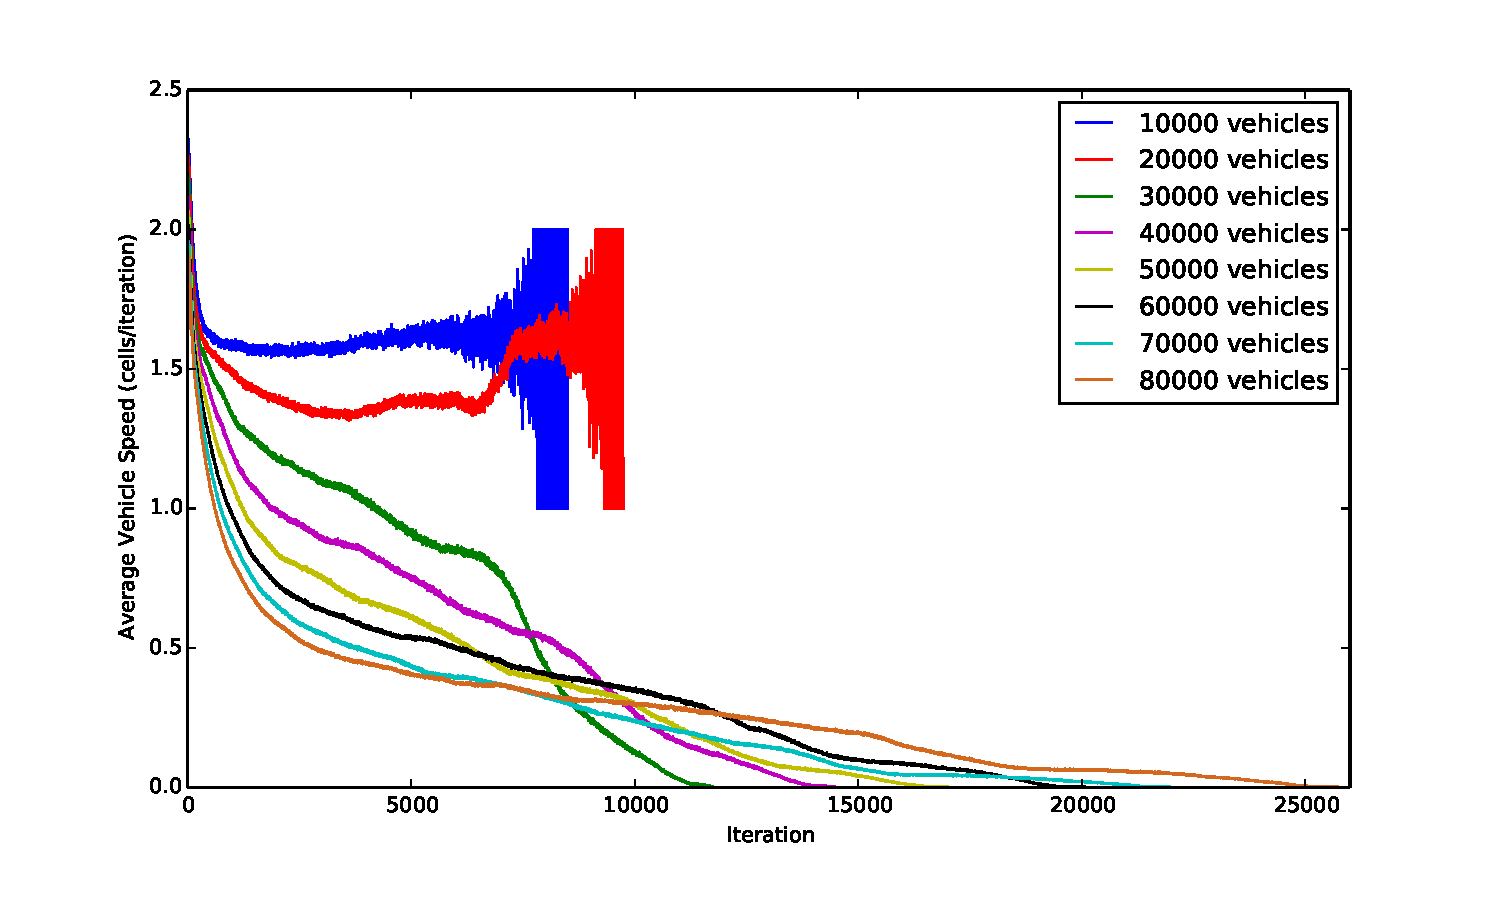
\includegraphics[width=0.9\textwidth]{dijkstra-speed}
    \caption{Average speed at each iteration for vehicles routing with
    Dijkstra's Algorithm}\label{fig:dijkstra-speed}
\end{figure}

The graph in Figure \ref{fig:dijkstra-speed} shows two different outcomes when
routing with Dijkstra's Algorithm. When simulating with 10,000 and 20,000
vehicles, we see the behaviour of the algorithm when all vehicles reach their
destination and terminate successfully. The remaining six simulations show the
behaviour of the algorithm when it fails to terminate and the vehicles slow to a
halt.

\begin{wrapfigure}{l}{0.4\textwidth}
    \vspace{-1em}
    \begin{greybox}
        \centering
        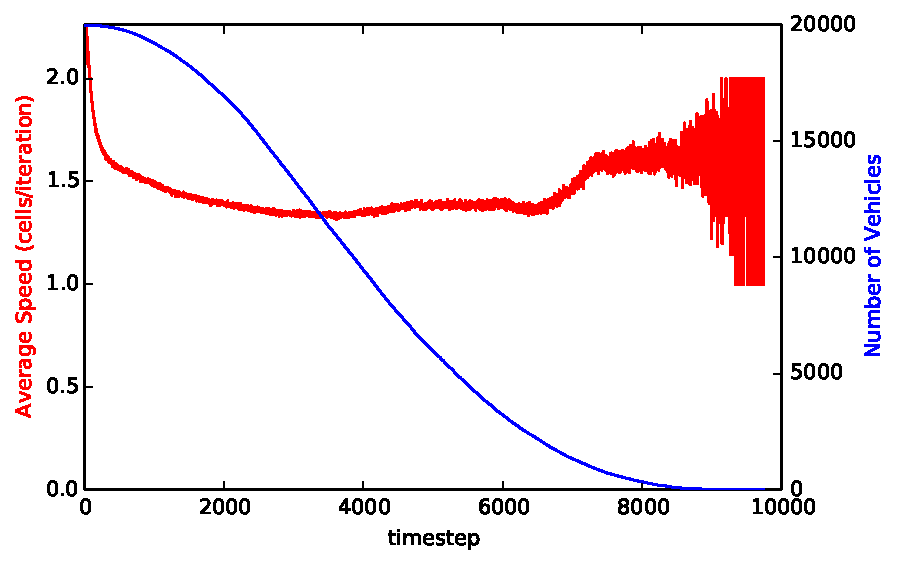
\includegraphics[width=\textwidth]{20k-dij-speed}
        \caption{Comparison of speed and remaining number of vehicles using
        Dijkstra's algorithm with 20,000 vehicles.}\label{fig:20k-dij-speed}
    \end{greybox}
    \vspace{-2em}
\end{wrapfigure}

In the successful termination cases, we see three stages. The average speed
starts high, followed by a decline as we reach the congested state. This is
followed by a longer period of time where the speed remains mostly stable whilst
the vehicles move slowly towards their destinations. Finally, we see a period
with increased speed volatility.  This is due to the decreased volume of
vehicles causing the average to change much faster, as can be seen in Figure
\ref{fig:20k-dij-speed}.

In the case of simulations that do not terminate normally, we see the same first
two stages (pre-congestion and congestion), but at a certain
inflection point the average speed declines faster until it reaches zero. This
is most notable for the 30,000 vehicle case, where the inflection point can be
seen at around iteration 7,000, after which the average speed enters a steep
decline.

The cause of the simulation failure can be seen in Figure \ref{fig:dijkstra-wtf}
- the Elephant \& Castle roundabout in central London becomes fully congested,
stopping any vehicle from being able to route past the roundabout. As the queue
of cars continues to grow, more and more main roads become full until no
remaining vehicles are capable of movement.

\begin{figure}[h]
\centering
\begin{subfigure}[b]{0.4\textwidth}
    \centering
    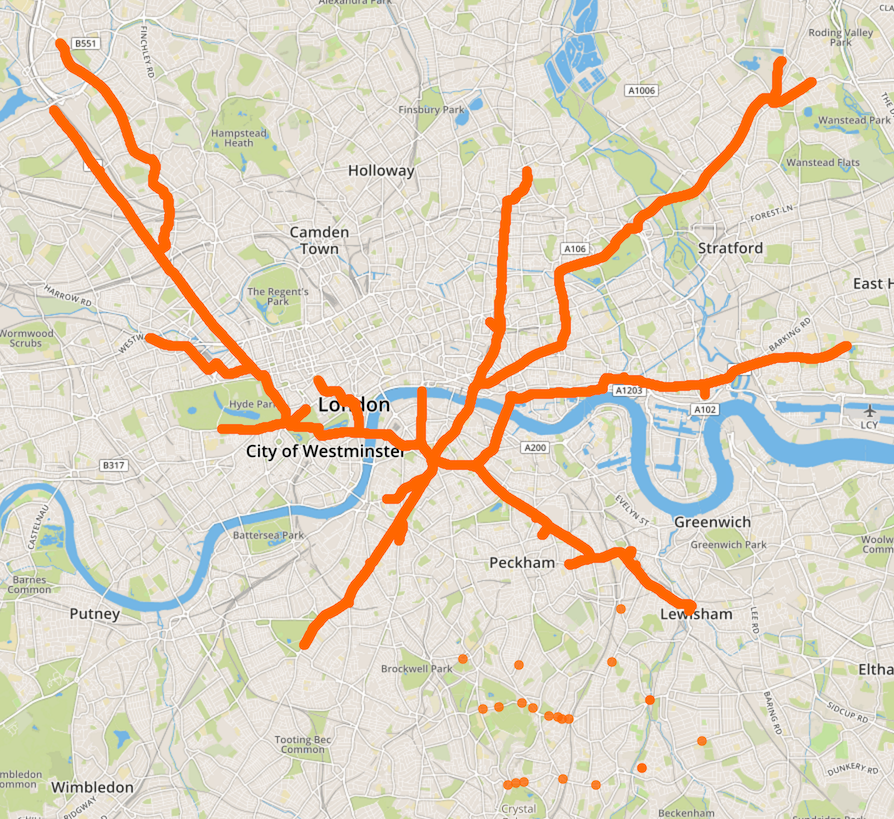
\includegraphics[height=13em]{dij-60k-blocked-wide}
\end{subfigure}
\hspace{1em}
\begin{subfigure}[b]{0.4\textwidth}
    \centering
    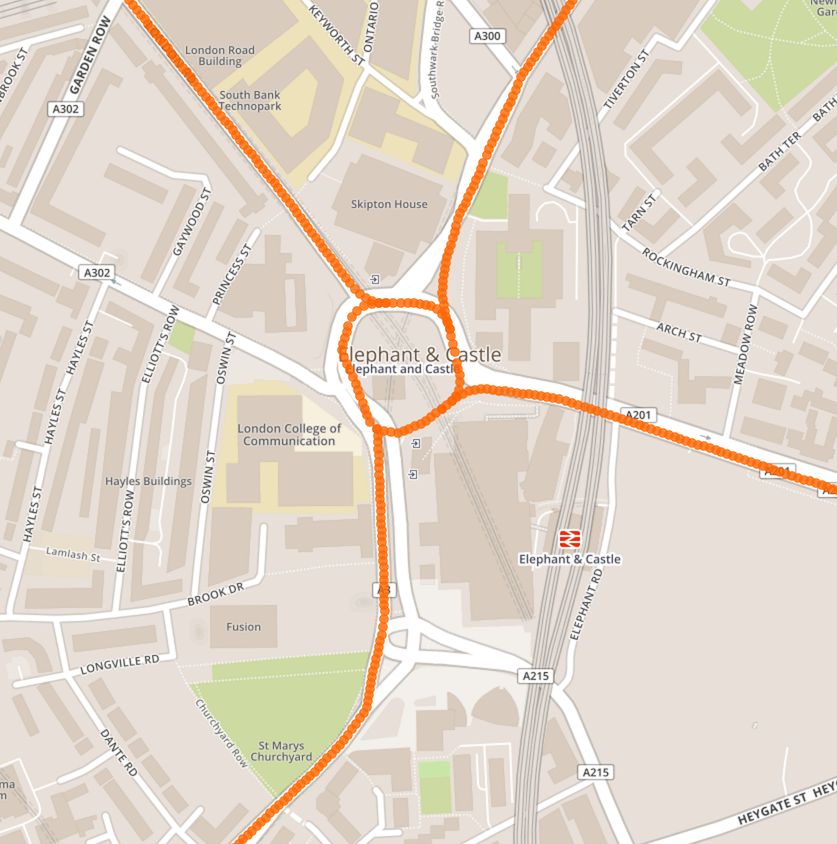
\includegraphics[height=13em]{dij-60k-blocked-close}
\end{subfigure}
\caption{The system state shortly before termination}\label{fig:dijkstra-wtf}
\end{figure}

\subsection{Marmoset Algorithm}\label{sec:marmoset-eval}

\begin{figure}[p]
    \centering
    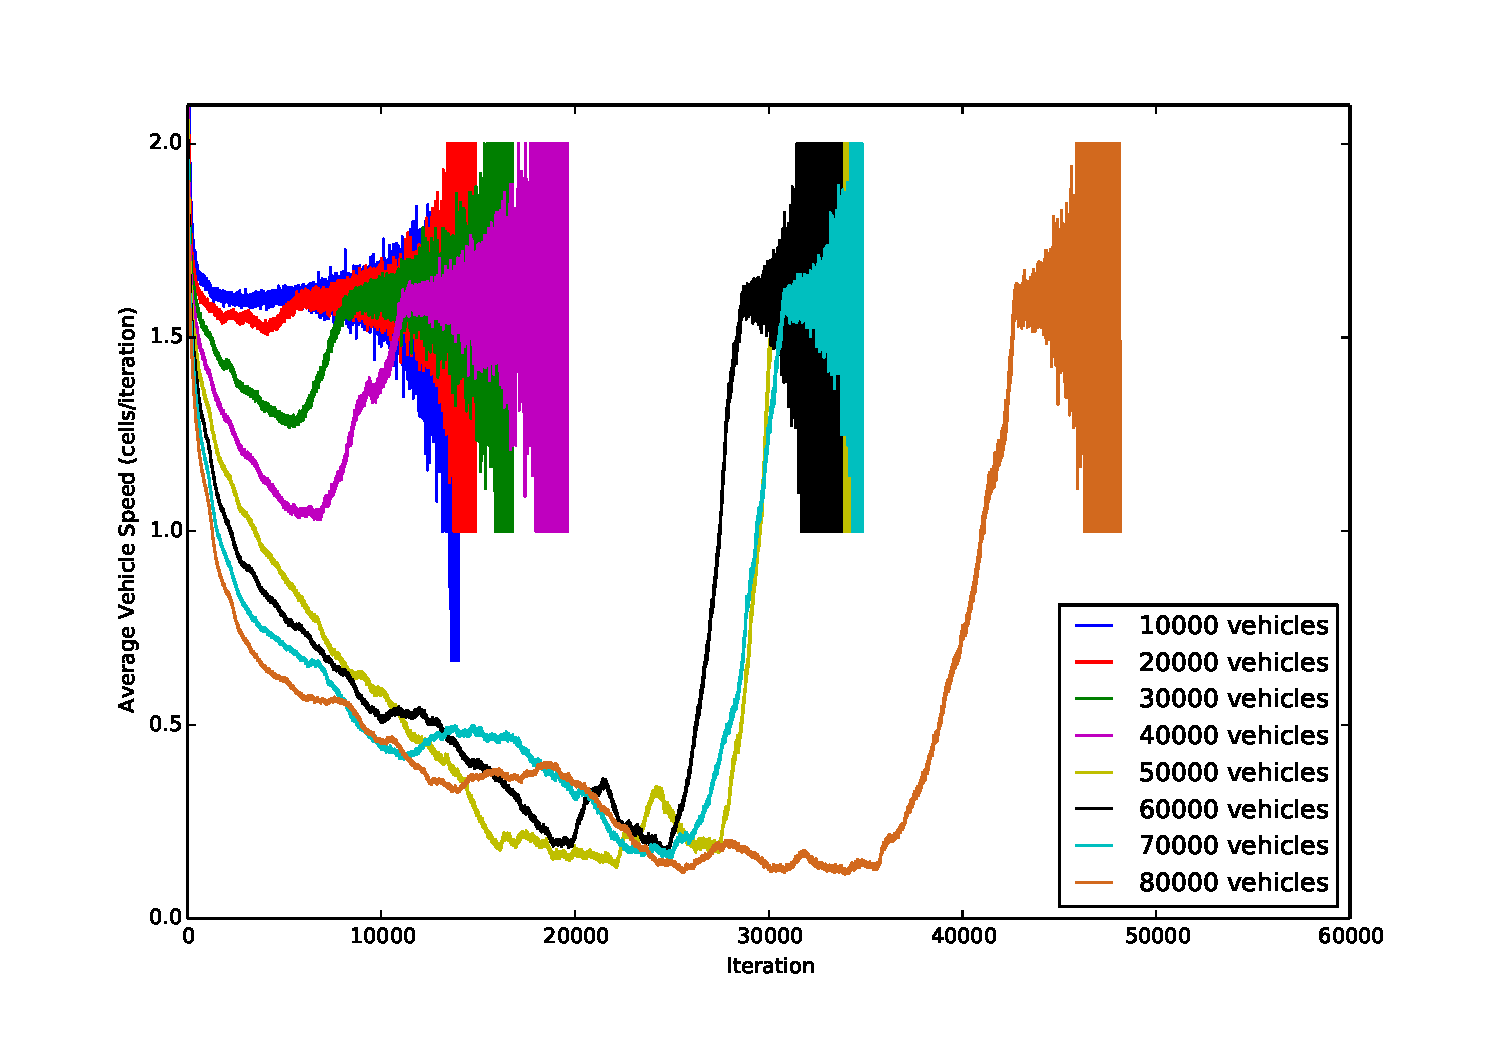
\includegraphics[width=0.9\textwidth]{sdv-speed}
    \caption{Average speed at each iteration for vehicles routing with the Marmoset Algorithm}\label{fig:sdv-speed}
\end{figure}

\begin{figure}[p]
    \centering
    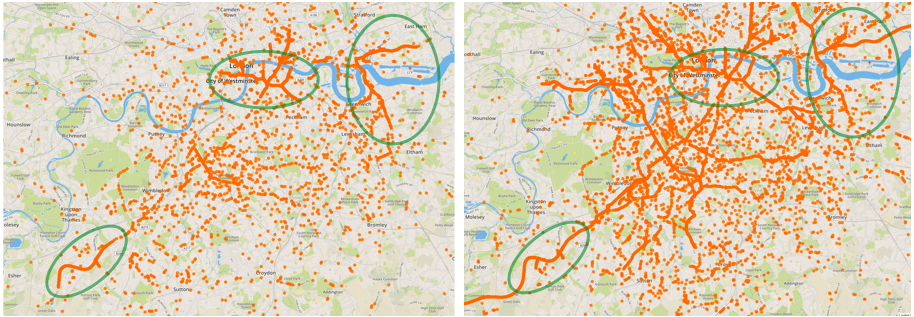
\includegraphics[width=0.8\textwidth]{i11k-sdv-comparison}
    \caption{The 11,000th iteration of 50,000 and 80,000 vehicles respectively.}\label{fig:i11k-congestion}
\end{figure}

\begin{figure}[p]
    \centering
    \begin{subfigure}[b]{0.3\textwidth}
        \centering
        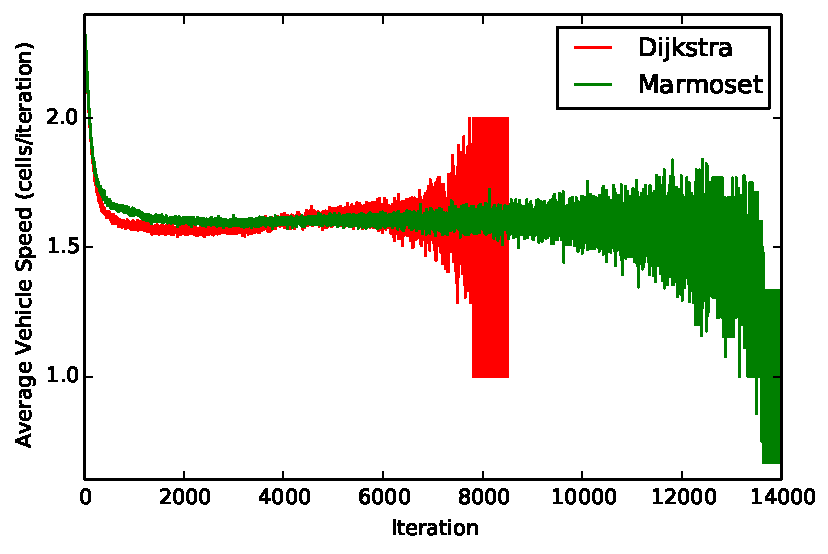
\includegraphics[width=\textwidth]{sdv-dij-comp-10k}
        \caption{10,000 vehicles}
    \end{subfigure}
    \begin{subfigure}[b]{0.3\textwidth}
        \centering
        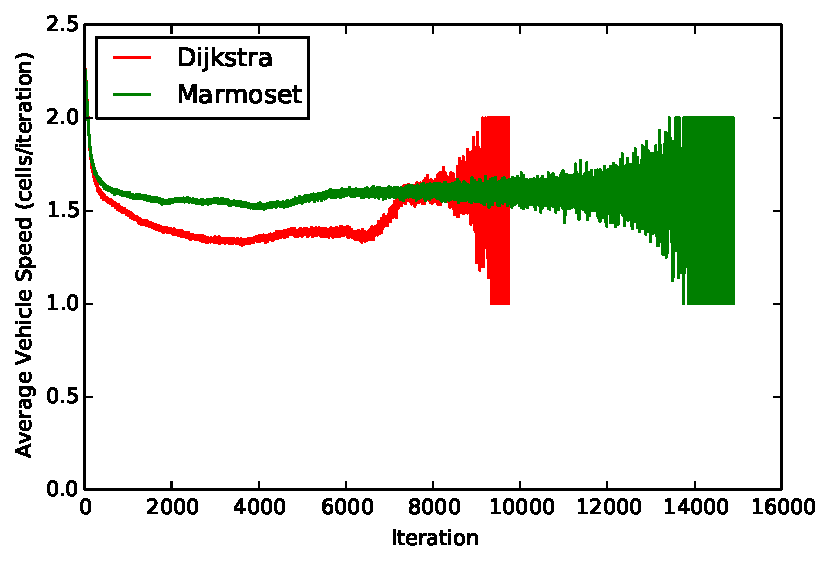
\includegraphics[width=\textwidth]{sdv-dij-comp-20k}
        \caption{20,000 vehicles}
    \end{subfigure}
    \begin{subfigure}[b]{0.3\textwidth}
        \centering
        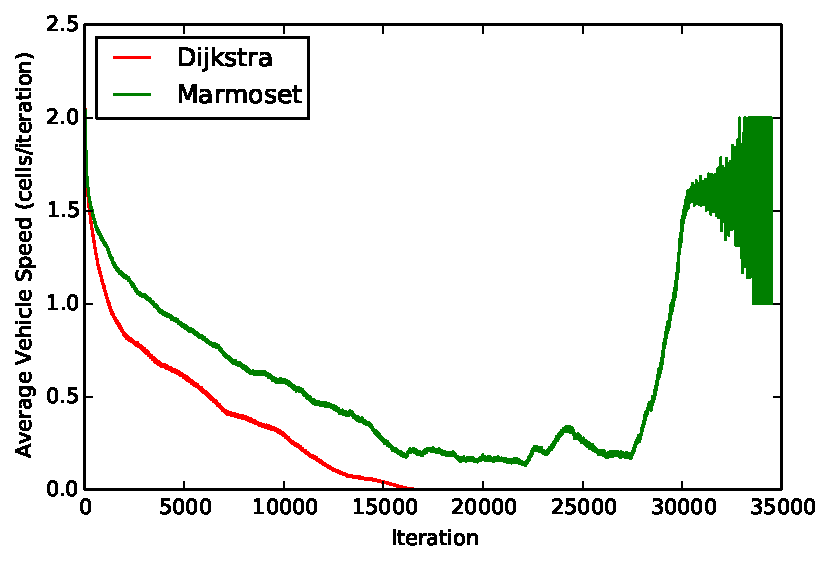
\includegraphics[width=\textwidth]{sdv-dij-comp-50k}
        \caption{50,000 vehicles}
    \end{subfigure}
    \caption{Comparison of average speed between Dijkstra's algorithm and the Marmoset algorithm}\label{fig:sdv-dij-comp}
\end{figure}

We now compare these results to the Marmoset routing algorithm. The most notable
difference is that the Marmoset algorithm successfully terminates even when
simulating 80,000 vehicles entering the city centre, 16,000 more than in rush
hour.

Figure \ref{fig:sdv-speed} shows that the Marmoset algorithm exhibits the same
behaviour as Dijkstra's Algorithm for 10,000 and 20,000 vehicles, but without
the limitation on the number of vehicles that can be simulated. The data shows
the same three stage behaviour as before, with the congested stage elongating as
the number of vehicles increases. We can also see a large difference in the
amount of time it takes for the simulation to terminate, falling into three
separate clusters - less than 40,000 vehicles, 50,000 to 70,000 vehicles and
80,000 vehicles. The reason for this is not clear from this graph alone. To gain
further insight into why this clustering may be occuring, we can look directly
at the state of the vehicles at specific iterations.

The engine records a snapshot of the position of each vehicle every 1000
iterations. We will compare the state of the system when simulating 50,000
vehicles and 80,000 vehicles, at iteration 11,000. This has been chosen as it is
approximately at the inflection point where the vehicles enter their most
congested state with the slowest average speed. However, the 80,000 vehicle
iteration takes significantly longer to leave this state than the 50,000 vehicle
simulation.

Figure \ref{fig:i11k-congestion}, helps us understand what the cause of this
behaviour may be. For the 50,000 vehicle simulation, we see three key areas of
congestion (circled in green on both maps). For the lower density simulation,
these three areas are separated - once a vehicle has left the congested roads it
enters an area of low congestion. In the 80,000 vehicle simulation, this is not
the case - instead, the highly congested roads are joined together, requiring
significantly longer to clear.  We can conclude that the clustering of total
travel time is a property of the map and routes that run on it - as the number
of vehicles on the road increases, areas prone to congestion increase in size
and connect, causing sudden jumps in completion time with only a small increase
in the number of vehicles.

Figure \ref{fig:sdv-dij-comp} shows a direct comparision between the two
algorithms. We see that when Dijkstra's algorithm does terminate, vehicles reach
their destinations earlier than with the Marmoset algorithm, despite a lower
average speed. This is likely due to the `selfish' behaviour of Dijkstra's
algorithm, allowing certain vehicles to reach their destinations earlier. With
lower vehicles densities, this frees up the roads and enables other vehicles to
reach their destinations sooner. However, with more vehicles on the road the
congestion blocks vehicles from reaching their destination.

\subsection{Per-Vehicle Metrics}

The data above shows what happens to the vehicles on average, but does not
provide us with any further insight on the distribution of speed or congestion.
The vehicle metrics can be used to better understand the impact each algorithm
has on travel time for each vehicle.

\begin{figure}[h]
    \centering
    \begin{subfigure}[b]{0.23\textwidth}
        \centering
        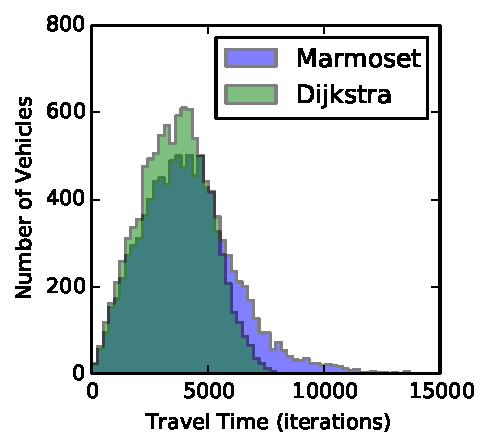
\includegraphics[width=\textwidth]{tt-10k}
        \caption{10,000 vehicles}\label{fig:tt-hist-10k}
    \end{subfigure}
    \begin{subfigure}[b]{0.23\textwidth}
        \centering
        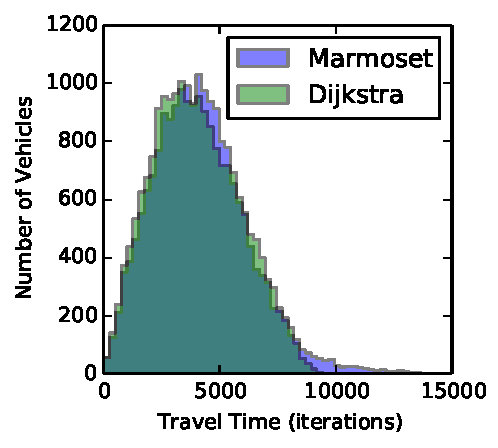
\includegraphics[width=\textwidth]{tt-20k}
        \caption{20,000 vehicles}\label{fig:tt-hist-20k}
    \end{subfigure}
    \begin{subfigure}[b]{0.23\textwidth}
        \centering
        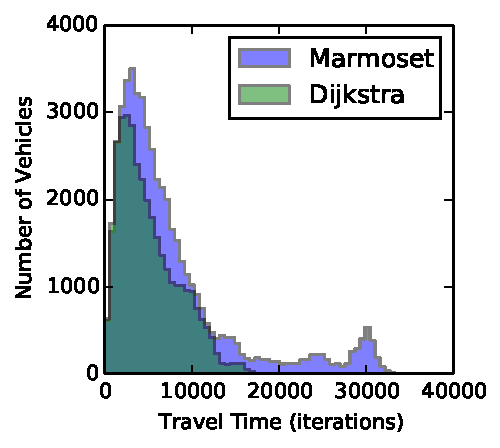
\includegraphics[width=\textwidth]{tt-50k}
        \caption{50,000 vehicles}\label{fig:tt-hist-50k}
    \end{subfigure}
    \begin{subfigure}[b]{0.23\textwidth}
        \centering
        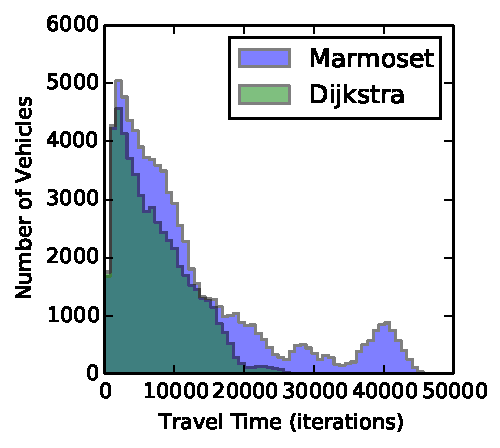
\includegraphics[width=\textwidth]{tt-80k}
        \caption{80,000 vehicles}\label{fig:tt-hist-80k}
    \end{subfigure}
    \caption{Histogram comparing travel time of vehicles using each algorithm.}\label{fig:tt-hist}
\end{figure}

In Figure \ref{fig:tt-hist}, we see some interesting patterns emerge. As
demonstrated by the graphs comparing average speed, lower density simulations
complete faster using Dijkstra's algorithm. In Figure \ref{fig:tt-hist-10k}
this behaviour is particularly noticable, with the Marmoset algorithm showing a
tail of vehicles with long travel times, although this is less noticable in
Figure \ref{fig:tt-hist-20k}.

Figure \ref{fig:tt-hist-50k} gives us further insight into the clustering of
completion times mentioned above (see Figure \ref{fig:sdv-speed}). On the
right of the histogram we see a small spike in travel times, centred around
iteration 30,000. This supports the theory that congested areas become
connected and dependent on each other for vehicles to reach their destinations -
once a certain group of vehicles reach their destinations, the group they
`blocked' is able to move once again. The same observation can be made with
Figure \ref{fig:tt-hist-80k}, which has a small spike at iteration 30,000 and
another, larger spike around iteration 40,000.

\subsection{Vehicle Ratio Analysis}

In addition to comparison between the two routing algorithms, we can also
analyse their behaviour when driving together on the same roads. As shown in
Section \ref{sec:density}, routing using only Dijkstra's algorithm fails to
terminate with more than 20,000 vehicles. One of the issues with multi-vehicle
routing algorithms is that in order to improve congestion some vehicles have to
take longer routes than they otherwise would have. Human drivers may not
appreciate being told to take a longer route than they would otherwise use. We
can analyse the effects of this behaviour by running both types of vehicle on
the road at the same time and identify what percentage of vehicles have to be
`misbehaving' for the algorithm to fail.

\begin{figure}[h]
    \centering
    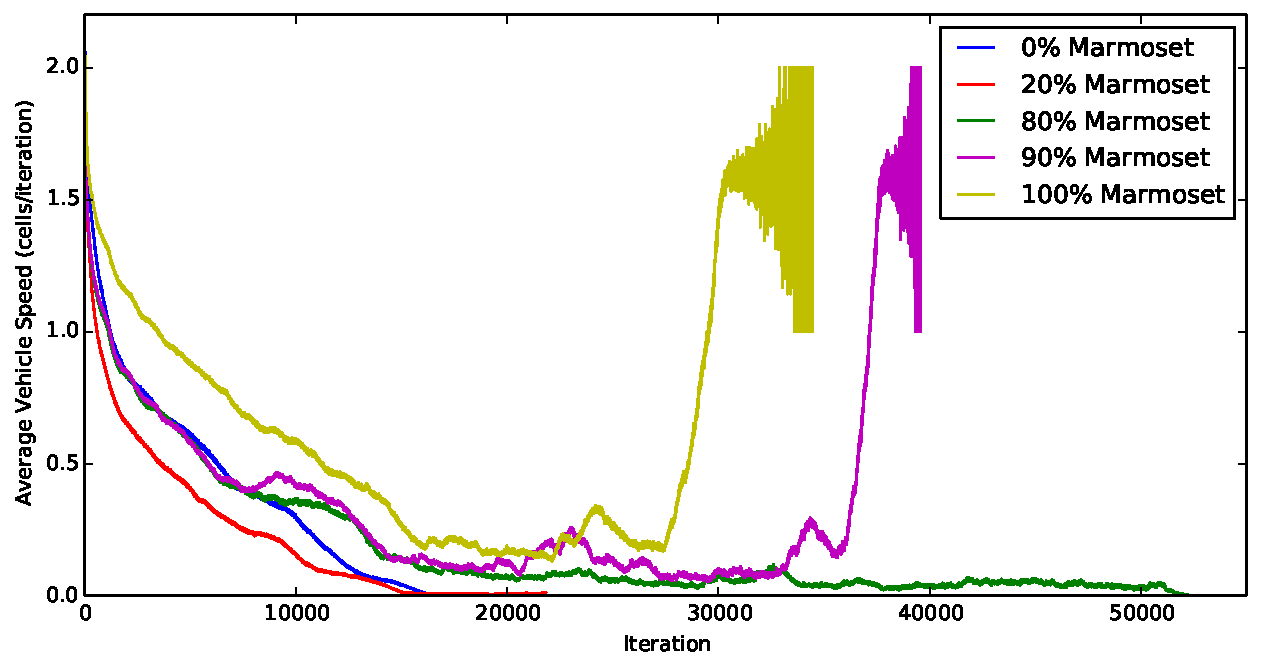
\includegraphics[width=0.8\textwidth]{ratio-av.pdf}
    \caption{Average velocity simulating 50,000 vehicles using the Marmoset and Dijkstra's algorithm.}\label{fig:ratio-av}
\end{figure}

Simulating 50,000 vehicles with different vehicle densities showed how strong
the impact even a small number of non-Marmoset vehicles could have on
congestion. Surprisingly, even with 80\% of the vehicles using the Marmoset
algorithm, the simulation failed to terminate. Figure \ref{fig:ratio-av} shows
the average speed of the vehicles when using both algorithms simultaneously in
various combinations. Although the vehicles fail to reach their destinations
completely with 80\% Marmoset vehicles, we do see a change in the behaviour of
the algorithm as the proportion of Marmoset vehicles increases. Notably, the
time it takes for the average velocity to reach zero is drastically increased -
it took 52,801 iterations before the engine decided to terminate the simulation.

\begin{figure}[h]
    \centering
    \begin{subfigure}[b]{0.45\textwidth}
        \centering
        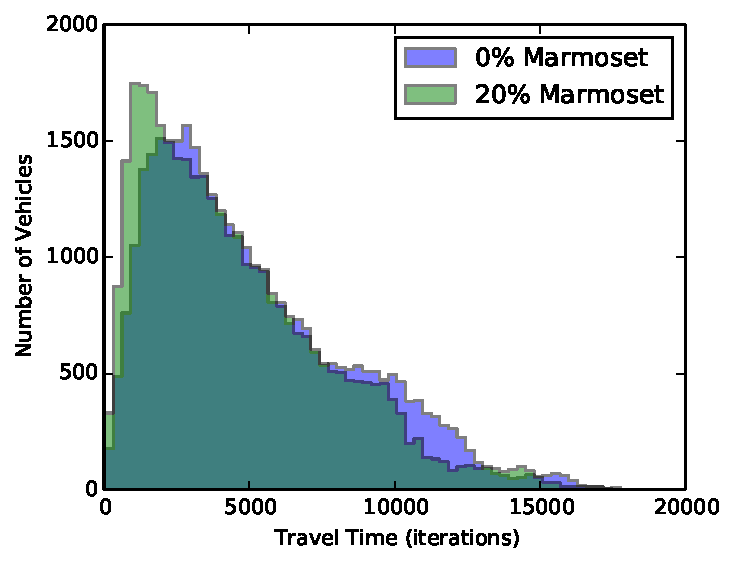
\includegraphics[width=\textwidth]{0-20-hist}
        \caption{}\label{fig:0-20-hist}
    \end{subfigure}
    \hfill
    \begin{subfigure}[b]{0.45\textwidth}
        \centering
        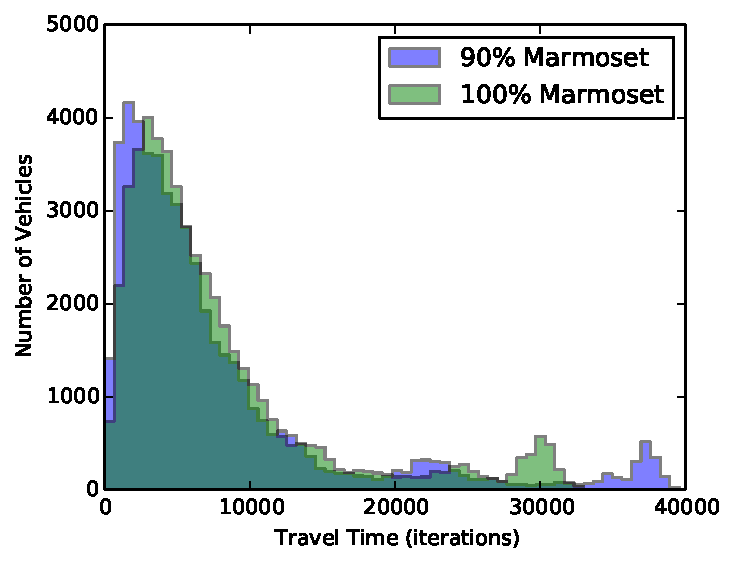
\includegraphics[width=\textwidth]{90-100-hist}
        \caption{}\label{fig:90-100-hist}
    \end{subfigure}
    \caption{Histograms of travel time for different ratios of vehicles.}\label{fig:ratio-hists}
\end{figure}

We also see changes in both average speed and total completion time with 90\%
Marmoset vehicles, even though all vehicles reach their destinations. The lack
of ability to operate effectively whilst routing with other types of vehicles is
a flaw in the algorithm that suggests it may not be appropriate for real world
use - any multi-vehicle routing algorithm would be rolled out slowly rather than
all at once, meaning it should be able to handle different types of vehicles on
the road. Interestingly, Figure \ref{fig:ratio-av} shows that average speed with
20\% Marmoset vehicles is significantly slower than when routing exclusively
with Dijkstra's algorithm.

However, the overall picture does not appear to be so simple. The histogram in
Figure \ref{fig:0-20-hist} shows that the vehicles that do reach their
destination do so sooner when there are some vehicles using the Marmoset
algorithm. One possible cause of this could be that the Marmoset vehicles avoid
the higher congestion areas, allowing the Dijkstra vehicles to reach their
destinations sooner. This could also explain the lower average speeds, as the
Marmoset vehicles would avoid the fastest roads, allowing the nearby Dijkstra
vehicles to move towards their destination with less congestion.

In Figure \ref{fig:90-100-hist}, we see the impact of vehicles using the most
congested routes on overall travel time. Notably, the peak of the 90\% histogram
occurs earlier than for the 100\% histogram, but it has a longer tail with a
spike around 8,000 iterations later. This is likely due to the Dijkstra vehicles
causing a further increase in congestion for busy roads, excaberating the
congestion connectivity issue discussed in Section \ref{sec:marmoset-eval}.

\subsection{Algorithm Performance}

The Marmoset algorithm must be fast enough to return routing queries in real-time
whilst vehicles are on the road. We will now analytically derive the asymptotic
peformance of the algorithm.

We will start by defining the number of vehicles as $N$ and the number of
iterations as $I$ (note that this will not be known in advance and could be
infinite). Dijkstra's algorithm runs in $O(E \log V)$ when using a binary heap for the
priority queue, which is how it is implemented in GraphHopper. The vehicles that
route themselves with Dijkstra's algorithm calculate their route once during
their first iteration and then simply iterate through their route until reaching
their destination. This means that the first timestep for each vehicle takes
$O(E\log V)$ and every subsequent timestep is $O(1)$. Hence for all vehicles, we
have a worst case performance of $O(NE\log V))$. For the overall system, we
have that as $I \rightarrow \infty$, the performance of the simulation overall
tends to $O(IN)$. We also have a substantial performance improvement through the
use of Contraction Hierarchies, analysed in~\cite{ch-complexity}.

For the Marmoset algorithm, a certain percentage of the vehicles are re-routed
every iteration - let this value be $c$. This means that the average runtime
iteration is $O(cNE\log V)$, which is equivalent to $O(NE \log V)$. The
rebuilding of the Expected Map takes $O(N)$, which is less than the routing step
and hence the runtime of the whole system is $O(INE\log V)$. We are also
limited by the fact that we cannot use Contraction Hierarchies, as the algorithm
re-weights the edegs on the graph each time the Expected Map is recalculated.

Clearly, the performance of the Marmoset algorithm is worse than routing using
Dijkstra's algorithm. This was shown to be true in practice, with the Dijkstra's
simulation taking around 15 minutes compared to up to 5 hours for the Marmoset
algorithm. However, there are many ways this could be improved in the real
world. When simulating, all routing requests must be performed on a single
machine - in the real world, the Expected Map could be stored centrally and
distributed the vehicles, who then perform their own requests. This reduces the
performance of the centralised system to $O(N)$ per iteration, with each vehicle
running Dijkstra's algorithm in $O(E\log V)$. As routing is a task many GPS
systems are already do, this seems to be a realistic option for implementing the
algorithm in the real world. Furthermore, it is likely that the code and
algorithms could be substantially opimised to improve performance were a central
system a requirement.

\subsection{Algorithm Limitations}

The approach chosen does have a few limitations. Other than speed, there are a
few other things missing that could improve the efficiency of the routes
generated by the algorithm.

The algorithm's parameters - the progress function, congestion function, damping
factor and re-route percentage - were chosen based on brief analysis of a
running simulation rather than in depth exploration of the effect changing the
parameters. This would offer further insight into the working of the algorithm
as well as improving its performance overall. Unfortunately this was not
possible due to the large number of possible combinations of parameters as well
as the longer running time for simulations using the Marmoset algorithm.

A key factor that the Expected Map does not take account of is the time at which
a vehicle will travel on a particular road. If a large number of vehicles were
all travelling along the same route but at different times, the Expected Map
would believe that the road would be congested in spite of this. The progress
function was added to mitigate this, but it does not completely eradicate the
issue.

We also saw some issuse regarding increased travel time

* large increases in travel time for some vehicles +

\section{Simulation Engine Evaluation}

We will now analyse how well the simulation engine has performed in terms
of its suitability for algorithm design.

\subsection{Flexibility}

Thanks to the system's architecture, implementing and testing the Marmoset
algorithm has been a painless task, enabling insight though both visualisation
and data analysis.

\subsection{Limitations}

* metric gathering improvement
* performance improvement
* labelling different types of vehicles in the UI
* V2V comms
* show planned routes
* 'higher level' visualisation stuff

BUT: don't wanna fall prey to the same issues with MATSim -> more like SUMO for
cities.

%{\bf A topic-specific chapter, of roughly $15$ pages}
%\vspace{1cm}

%\noindent
%This chapter is intended to evaluate what you did.  The content is highly
%topic-specific, but for many projects will have flavours of the following:

%\begin{enumerate}
%\item functional  testing, including analysis and explanation of failure
      %cases,
%\item behavioural testing, often including analysis of any results that
      %draw some form of conclusion wrt. the aims and objectives,
      %and
%\item evaluation of options and decisions within the project, and/or a
      %comparison with alternatives.
%\end{enumerate}

%\noindent
%This chapter often acts to differentiate project quality: even if the work
%completed is of a high technical quality, critical yet objective evaluation
%and comparison of the outcomes is crucial.  In essence, the reader wants to
%learn something, so the worst examples amount to simple statements of fact
%(e.g., ``graph X shows the result is Y''); the best examples are analytical
%and exploratory (e.g., ``graph X shows the result is Y, which means Z; this
%contradicts [1], which may be because I use a different assumption'').  As
%such, both positive {\em and} negative outcomes are valid {\em if} presented
%in a suitable manner.

% -----------------------------------------------------------------------------

\chapter{Conclusion}
\label{chap:conclusion}

This section will conclude the project, discussing the overall quality of the
algorithm and simulation engine before discussing the potential they hold for
future research and development.

\section{Achievements and Contributions}

The primary achievement of this project was building a simulation engine focussed
on algorithm design that is fast enough to handle the simulation of entire cities.
The simulation engine was then used to design, implement and optimise the
Marmoset algorithm for multi-vehicle routing.

The architecture of the simulation engine enabled easy implementation of a
reasonably complex algorithm for routing. The three main architectural insights
were the separation of Vehicle and VehicleIterator classes, the use of an event
system for adding behaviour and taking advantage of the flexibility of the
GraphHopper routing engine.

The engine was then optimised for speed and ease of use. Running a 64,000
vehicle simulation took just 6 minutes 24 seconds when using routes provided by
Dijkstra's algorithm, or 20.3ms per iteration when performing offline routing.
It also offers a responsive interface for the visualisation of vehicles whilst
the simulation is in progress.

Following research into existing algorithms, a novel approach to providing
routes for multiple vehicles was designed and implemented. By using the insight
from the BeeJamA algorithm, a congestion function was identified and optimised,
providing a key metric in predicting a vehicle's expected velocity. The use of
visualisation whilst simulating enabled fast iteration and improvement on this
function as well as quick insight into the impact this had on congestion
overall. In conjunction with post-simulation visualisation, this also led to
identifying the need for the progress function, avoiding overpenalising busy but
distant roads.

\section{The Marmoset Algorithm}

As shown in the Critical Evaluation (Chapter \ref{chap:evaluation}), the
Marmoset algorithm performed better than Dijkstra's for situations with high
levels of congestion. Empirical analysis demonstrated that the algorithm offered
an improvement in average speed and avoided mass congestion when dealing with
high volumes of vehicles. It was also showon to be able to handle a small number
of `selfish' vehicles driving alonside the Marmoset routed vehicles.

However, there were some flaws that would need addressing in future research.
Improvements to travel time

Nonetheless, the approach has shown promise, and is flexible enough to cover
many other potential situations. For example, ...

Although the algorithm has some minor flaws that could be improved upon, it is
able to solve the multi-vehicle routing problem in a novel and effective manor.

Extensions:
* support road closure/roadworks etc in the expected map
* multi-directional edge blocking!

\section{The Marmoset Simulation Engine}

The simulation engine is


%{\bf A compulsory chapter,     of roughly $5$ pages}
%\vspace{1cm}

%\noindent
%The concluding chapter of a dissertation is often underutilised because it
%is too often left too close to the deadline: it is important to allocation
%enough attention.  Ideally, the chapter will consist of three parts:

%\begin{enumerate}
%\item (Re)summarise the main contributions and achievements, in essence
      %summing up the content.
%\item Clearly state the current project status (e.g., ``X is working, Y
      %is not'') and evaluate what has been achieved with respect to the
      %initial aims and objectives (e.g., ``I completed aim X outlined
      %previously, the evidence for this is within Chapter Y'').  There
      %is no problem including aims which were not completed, but it is
      %important to evaluate and/or justify why this is the case.
%\item Outline any open problems or future plans.  Rather than treat this
      %only as an exercise in what you {\em could} have done given more
      %time, try to focus on any unexplored options or interesting outcomes
      %(e.g., ``my experiment for X gave counter-intuitive results, this
      %could be because Y and would form an interesting area for further
      %study'' or ``users found feature Z of my software difficult to use,
      %which is obvious in hindsight but not during at design stage; to
      %resolve this, I could clearly apply the technique of Smith [7]'').
%\end{enumerate}

% =============================================================================

% Finally, after the main matter, the back matter is specified.  This is
% typically populated with just the bibliography.  LaTeX deals with these
% in one of two ways, namely
%
% - inline, which roughly means the author specifies entries using the
%   \bibitem macro and typesets them manually, or
% - using BiBTeX, which means entries are contained in a separate file
%   (which is essentially a databased) then inported; this is the
%   approach used below, with the databased being dissertation.bib.
%
% Either way, the each entry has a key (or identifier) which can be used
% in the main matter to cite it, e.g., \cite{X}, \cite[Chapter 2}{Y}.

\backmatter

\bibliography{dissertation}

% -----------------------------------------------------------------------------

% The dissertation concludes with a set of (optional) appendicies; these are
% the same as chapters in a sense, but once signaled as being appendicies via
% the associated macro, LaTeX manages them appropriatly.

\appendix

\chapter{Self-Driving Vehicle Implementation}
\label{appx:example}

%Content which is not central to, but may enhance the dissertation can be
%included in one or more appendices; examples include, but are not limited
%to

%\begin{itemize}
%\item lengthy mathematical proofs, numerical or graphical results which
      %are summarised in the main body,
%\item sample or example calculations,
      %and
%\item results of user studies or questionnaires.
%\end{itemize}

%\noindent
%Note that in line with most research conferences, the marking panel is not
%obliged to read such appendices.

% =============================================================================

\end{document}
